%
% FH Technikum Wien
% !TEX encoding = UTF-8 Unicode
%
% Erstellung von Master- und Bachelorarbeiten an der FH Technikum Wien mit Hilfe von LaTeX und der Klasse TWBOOK
%
% Um ein eigenes Dokument zu erstellen, müssen Sie folgendes ergänzen:
% 1) Mit \documentclass[..] einstellen: Master- oder Bachelorarbeit, Studiengang und Sprache
% 2) Mit \newcommand{\FHTWCitationType}.. Zitierstandard festlegen (wird in der Regel vom Studiengang vorgegeben - bitte erfragen)
% 3) Deckblatt, Kurzfassung, etc. ausfüllen
% 4) und die Arbeit schreiben (die verwendeten Literaturquellen in Literature.bib eintragen)
%
% Getestet mit TeXstudio mit Zeichenkodierung ISO-8859-1 (=ansinew/latin1) und MikTex unter Windows
% Zu beachten ist, dass die Kodierung der Datei mit der Kodierung des paketes inputenc zusammen passt!
% Die Kodierung der Datei twbook.cls MUSS ANSI betragen!
% Bei der Verwendung von UTF8 muss dnicht nur die Kodierung des Dokuments auf UTF8 gestellt sein, sondern auch die des BibTex-Files!
%
% Bugreports und Feedback bitte per E-Mail an latex@technikum-wien.at
%
% Versionen
% *) V0.7: 9.1.2015, RO: Modeline angepasst und verschoben
% *) V0.6: 10.10.2014, RO: Weitere Anpassung an die UK
% *) V0.5: 8.8.2014, WK: Literaturquellen überarbeitet und angepasst
% *) V0.4: 4.8.2014, WK: Initalversion in SVN eingespielt
%
\documentclass[MMR,Master,english]{twbook}
\usepackage[utf8]{inputenc}
\usepackage[T1]{fontenc}
%
% Hier biblatex & Biber konfigurieren; Vergessen Sie nicht, dass Sie biber verwenden müssen um eine Bibliothek zu erzeugen
%
\usepackage[backend=biber, style=numeric, sorting=none]{biblatex}
\addbibresource{Literature.bib}
%
% Bei Bedarf bitte hier die Syntax-Highlightings anpassen
%
% own 
\usepackage{hyperref}
\usepackage{float}
\usepackage{comment}
\usepackage{csquotes}
\usepackage{pgfplots}
\usepackage{soul}
\usepackage{color}
\usepackage{xcolor}  % Required for custom colors
\sethlcolor{blue}
\setcounter{secnumdepth}{3} % in text 
\setcounter{tocdepth}{3} % contents
\usepackage{longtable}
\usepackage{pdflscape}
\usepackage{rotating}
\usepackage{tikz}
\usepackage{setspace}
\usetikzlibrary{shapes,arrows}
\usetikzlibrary{positioning}

\hypersetup{
    colorlinks=true, % Aktiviert farbige Links
    linkcolor={rgb,255:red,0;green,0;blue,255}, % Interne Links (z.B. Sections)
    citecolor=orange, % Zitate
    urlcolor={rgb,255:red,128;green,0;blue,128} % URLs
}

%
% Platzierungsoptionen 
%
\usepackage[final]{listings}
\lstset{captionpos=b, numberbychapter=false,caption=\lstname,frame=single, numbers=left, stepnumber=1, numbersep=2pt, xleftmargin=15pt, framexleftmargin=15pt, numberstyle=\tiny, tabsize=3, columns=fixed, basicstyle={\fontfamily{pcr}\selectfont\footnotesize}, keywordstyle=\bfseries, commentstyle={\color[gray]{0.33}\itshape}, stringstyle=\color[gray]{0.25}, breaklines, breakatwhitespace, breakautoindent}
\lstloadlanguages{[ANSI]C, C++, python, [gnu]make, gnuplot, Matlab}

%Formatieren des Quellcodeverzeichnisses
\makeatletter
% Setzen der Bezeichnungen für das Quellcodeverzeichnis/Abkürzungsverzeichnis in Abhängigkeit von der eingestellten Sprache
\providecommand\listacroname{}
\@ifclasswith{twbook}{english}
{%
    \renewcommand\lstlistingname{Code}
    \renewcommand\lstlistlistingname{List of Code}
    \renewcommand\listacroname{List of Abbreviations}
}{%
    \renewcommand\lstlistingname{Quellcode}
    \renewcommand\lstlistlistingname{Quellcodeverzeichnis}
    \renewcommand\listacroname{Abkürzungsverzeichnis}
}
% Wenn die Option listof=entryprefix gewählt wurde, Definition des Entyprefixes für das Quellcodeverzeichnis. Definition des Macros listoflolentryname analog zu listoflofentryname und listoflotentryname der KOMA-Klasse
\@ifclasswith{scrbook}{listof=entryprefix}
{%
    \newcommand\listoflolentryname\lstlistingname
}{%
}
\makeatother
\newcommand{\listofcode}{\phantomsection\lstlistoflistings}

% Die nachfolgenden Pakete stellen sonst nicht benötigte Features zur Verfügung
\usepackage{blindtext}
%
% Einträge für Deckblatt, Kurzfassung, etc.
%
\title{Virtualisierung eines Echtzeit-Betriebssystems zur Steuerung eines Roboters mit Schwerpunkt auf die
Einhaltung der Echtzeit}
\author{Halil Pamuk, BSc}
\studentnumber{51842568}
%\author{Titel Vorname Name, Titel\and{}Titel Vorname Name, Titel}
%\studentnumber{XXXXXXXXXXXXXXX\and{}XXXXXXXXXXXXXXX}
\supervisor{Sebastian Rauh, MSc. BEng}
%\supervisor[Begutachter]{Titel Vorname Name, Titel}
%\supervisor[Begutachterin]{Titel Vorname Name, Titel}
%\secondsupervisor{Titel Vorname Name, Titel}
%\secondsupervisor[Begutachter]{Titel Vorname Name, Titel}
%\secondsupervisor[Begutachterinnen]{Titel Vorname Name, Titel}
\place{Wien}
\kurzfassung{Erstellung einer Echtzeit-Robotersteuerungsplattform unter Verwendung von Salamander OS, Xenomai, QEMU
und PCV-522 in der Yocto-Umgebung. Die Plattform basiert auf Salamander OS und nutzt Xenomai für Echtzeit-
Funktionen. Dazu muss im ersten Schritt die Virtualisierungsplattform evaluiert werden. (QEMU, Hyper-V, Virtual
Box, etc.) Als weiterer Schritt folgt die Anbindung eines Roboters über eine VARAN-Bus Schnittstelle. Das
gesamte System wird in der Yocto-Umgebung erstellt und konfiguriert.
Das Hauptziel der Arbeit ist es, herauszufinden, wie die Integration von Echtzeit-Funktionen und effizienten
Kommunikationssystemen in eine Robotersteuerungsplattform die Reaktionszeit und Zuverlässigkeit von
Roboteranwendungen verbessern kann}
\schlagworte{Schlagwort1, Schlagwort2, Schlagwort3, Schlagwort4}
\outline{Sections~\ref{sec:salamander4-bare-metal} and~\ref{sec:salamander4-virtualization}  demonstrate the inital real-time latency values gathered for bare metal and virtualization. 
}
\keywords{Echtzeit, Virtualisierung, Xenomai, VARAN}
%\acknowledgements{\blindtext}

\begin{document}

\maketitle
%
% .. und hier beginnt die eigentliche Arbeit. Viel Erfolg beim Verfassen!
%
%Die folgende Gliederung von Bachelor- und Masterarbeiten ist für die Robotik-Studiengänge
%verpflichtend vorgeschrieben.
%
%- Deckblatt
%- Eidesstattliche Erklärung (digital signiert)
%- Kurzfassung und Abstract mit Schlüsselwörtern/Keywords
%- Danksagung (optional)
%- Inhaltsverzeichnis

%- Einleitung (die genannten Punkte müssen keine eigenen Unterkapitel sein, müssen aber aus der Einleitung klar hervorkommen):
%   - Stand der Technik
%   - Problem- und Aufgabenstellung
%   - Zielsetzung
%- Hauptteil -> Gliederung je nach Thema
%   - Methodik
%   - Resultate
%   - Wirtschaftliche Betrachtung (optional)
%   - Diskussion
%- Zusammenfassung und Ausblick

%- Literaturverzeichnis
%- Abbildungsverzeichnis
%- Tabellenverzeichnis
%- Abkürzungsverzeichnis (optional)
%- Glossar (optional)
%- Anhang (optional)

\chapter{Introduction}\label{cha:introduction}
In today's industrial production and automation, robot systems are well established and of crucial importance. Robots must react to their environment and perform time-critical tasks within strict time constraints. Delays or errors can have catastrophic consequences in some cases. Modern operating systems nowadays are categorized into two types:  general-purpose operating systems (GPOS) and real-time operating systems (RTOS). The key difference is whether the system is time-critical or not~\cite{canbazPerformanceAnalysisRealtime2022}. In a traditional GPOS, such as Windows or Linux-based distributions, a high-priority task cannot interrupt a kernel operation, as illustrated in Figure \ref{fig:kernel_generic}. This makes them not suitable for real-time requirements, as they cannot guarantee deterministic execution times.

\begin{figure}[H]
	\centering
	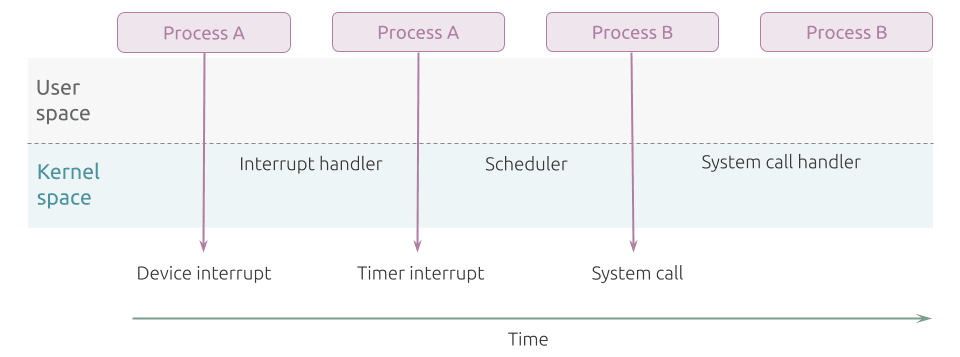
\includegraphics[width=0.75\columnwidth]{img/introduction/kernel_generic.png}
	\caption[Non-preemptible kernel]{Non-preemptible kernel \cite{WhatRealtimeLinuxa}}
	\label{fig:kernel_generic}
\end{figure}

\noindent However, in an RTOS, a high-priority process can interrupt a lower-priority task, even if it is in the middle of a kernel operation, as shown in Figure \ref{fig:kernel_rt} RTOS are specifically designed to react to events within fixed time limits and prioritise the execution of high-priority processes.

\begin{figure}[H]
	\centering
	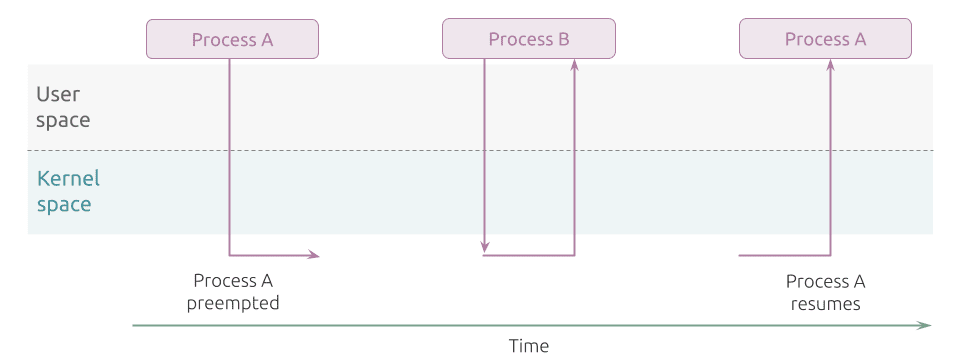
\includegraphics[width=0.75\columnwidth]{img/introduction/kernel_rt.png}
	\caption[Non-preemptible kernel]{Non-preemptible kernel \cite{WhatRealtimeLinuxa}}
	\label{fig:kernel_rt}
\end{figure}

\noindent Many Linux distributions can function as both GPOS and RTOS with kernel modifications.

\section{Real-Time Operating Systems}
\noindent The RTOS structure is visualized in Figure~\ref{fig:rtos_structure}.The core component of an RTOS that enables real-time capabilities is the kernel. It is responsible for managing system resources, scheduling tasks, and ensuring deterministic behavior \cite{malallahComprehensiveStudyKernel2021}. It employs preemptive scheduling mechanisms to allow high-priority tasks to preempt lower-priority tasks, ensuring that time-critical tasks are not delayed. Additionally, RTOS kernels are designed to allocate and manage memory resources efficiently and minimize interrupt latency, which is crucial for real-time applications that require immediate response to external events~\cite{wangRealtimeEmbeddedSystems2017}.

\begin{figure}[H]
	\centering
	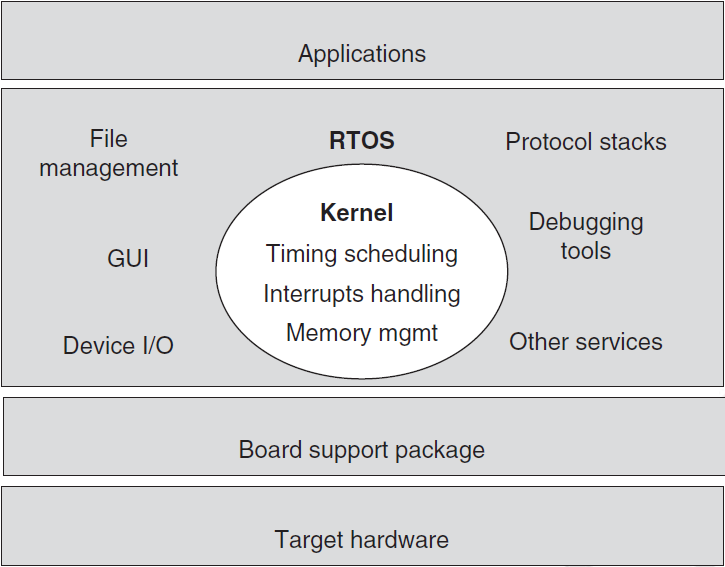
\includegraphics[width=0.50\columnwidth]{img/introduction/rtos_structure.png}
	\caption[RTOS Structure]{RTOS Structure~\cite{wangRealtimeEmbeddedSystems2017}}
	\label{fig:rtos_structure}
\end{figure}

\noindent In these real-time operating system, task scheduling is based on so-called priority-based preemptive scheduling~\cite{buttazzoHardRealtimeComputing2024}. Each task in a software application is assigned a priority. A higher priority means that a faster response is required. Preemptive task scheduling ensures a very fast response. Preemptive means that the scheduler can stop a currently running task at any point if it recognizes that another task needs to be executed immediately. The basic rule on which priority-based preemptive scheduling is based is that the task with the highest priority that is ready to run is always the task that must be executed. So if both a task with a lower priority and a task with a higher priority are ready to run, the scheduler ensures that the task with the higher priority runs first. The lower priority task is only executed once the higher priority task has been processed.

\bigskip \noindent Real-time systems are usually classified as either soft or hard real-time systems ~\cite{lipariRealTimeSchedulingHard}. The difference lies exclusively in the consequences of a violation of the time limits. Hard real-time is when the system stops operating if a deadline is missed, which can have catastrophic consequences. Soft real-time exists when a system continues to function even if it cannot perform the tasks within a specified time. If the system has missed the deadline, this has no critical consequences. The system continues to run, although it does so with undesirably lower output quality.

\section{Application Context}\label{sec:application_context}
This section briefly defines the context and scope within which this master's thesis was composed, highlighting the specific contributions and requirements set by SIGMATEK GmbH \& Co KG~\cite{pixelartSIGMATEKKompletteAutomatisierungssysteme}.

\begin{itemize}
	\item This work was written at SIGMATEK GmbH \& Co KG, a company that researches, develops, produces, and distributes automation technology for industrial machinery and plant engineering. SIGMATEK uses its own custom Linux-based operating system, to be run on their self-manufactured CPUs. This operating system will be referred to as ``Salamander 4'' in this work. The details of Salamander 4 are explained in Chapter~\ref{cha:salamander4}.
	\item Salamander 4 was created with Yocto~\cite{WelcomeYoctoProject}, an open-source project that helps develop custom Linux-based systems. Yocto is discussed in Section~\ref{sec:yocto}.
	\item Salamander 4 is virtualized through Quick emulator (QEMU), an open-source emulator and virtualizer that allows to run different operating systems on a computer QEMU is described in Section~\ref{sec:qemu}.
	\item Salamander 4 employs hard real-time with Xenomai 3~\cite{XenomaiXenomai}, a real-time framework for Linux that enables deterministic and low-latency performance. Xenomai 3 is detailed in Section~\ref{sec:xenomai}.
	\item The goal is to virtualize Salamander 4 and approach the performance of bare metal through real-time performance tunings, focussing on latency requirements set by SIGMATEK.
	      These modifications are subject of Chapter~\ref{cha:real-time_tuning}.
	\item The latency tool of the Xenomai suite to measure the scheduling latency of the real-time OS was suggested to use by SIGMATEK.
	\item SIGMATEK uses the VARAN bus for communication between machines and systems, a real-time Ethernet network that was specially developed for industrial automation. Its operating principle is outlined in Section \ref{sec:varan}.
	\item For the purpose of replacing the physical CPU, SIGMATEK provided a PCI Insert Card module PCV 522, that was plugged into the PC, as explained in Section \ref{sec:setup_experiment_virtualized}. This component could then be used to communicate with the Input/Output peripherals, just like the physical CPU could when the I/O modules were attached to it. Subsequently, the PCV 522 module of SIGMATEK was connected with the Pulse Width Module PW 022 of SIGMATEK over the VARAN bus and the VI 021 module of SIGMATEK serving as the power supply.
	\item The robotic application from Chapter \ref{cha:robotic_application} was written in Lasal Class 2, an object oriented programming tool of SIGMATEK with client-server technology and graphic representation.
\end{itemize}

\section{Related Work and State of the Art}
This master’s thesis builds upon a number of previous studies in the field of virtualization of real-time systems and the inherent latency. In this section, the most influential studies are presented and their relevance to the work is addressed.

\bigskip \noindent \citeauthor{perneelRealtimeCapabilitiesStandard2015} \cite{perneelRealtimeCapabilitiesStandard2015} mention in their work that Linux was initially developed as a general purpose operating system without real-time applications in mind. They talk about the evolution of real-time behavior in the standard Linux kernel and state that it has recently gained popularity among the real-time community, largely due to its open-source nature and stability. The authors explain how to transform Linux into a real-time operating system by implementing the PREEMPT-RT patches. The paper also emphasizes some kernel configurations that ensure that the system's real-time behavior is preserved during runtime. Even though these modifications to the kernel enable soft real-time performance, the authors underline the fundamental rule in real-time software, that latency improvements have a negative impact on throughput and kernel performance. This is due to the added overhead of the \texttt{CONFIG\_PREEMPT\_RT} option. They concluded with their Linux build and a testing application that Linux can be a viable option for real-time applications, if it is correctly configured. Similarly, \citeauthor{adamRealTimePerformanceResponse2021} \cite{adamRealTimePerformanceResponse2021} applied the PREEMPT\_RT patch on both Raspberry Pi 3 and BeagleBone Black and achieved significantly lower latencies compared to standard Linux kernels.

\bigskip \noindent In the course of writing this thesis, the white paper "Real-Time Performance Tuning Best Practice Guidelines for KVM-Based Virtual Machines" \cite{RealTimePerformanceTuning2022} by Intel has been instrumental. Given that the working computer used for this work is equipped with an Intel processor, the guidelines presented in this document were particularly relevant and valuable for optimizing real-time performance in KVM-based virtual machines. Chapter \ref{cha:real-time_tuning} contains an extensive tuning process, which involves configurations spanning the BIOS, kernel, host OS, QEMU/KVM virtualization layer, and the Salamander 4 OS itself. The document concludes that the described tuning methods effectively improve real-time performance for KVM-based VMs, even under heavy workloads.

\bigskip \noindent \citeauthor{yoonRealTimePerformanceAnalysis} \cite{yoonRealTimePerformanceAnalysis} use some of these real-time tunings in their research, including CPU shielding, memory locking, and spinning nanosleep, for controlling humanoid robots equipped with around 60 servo motors and sensors. They implement EtherCAT for real-time communication of distributed devices whereas this thesis uses Varan. The authors highlight the importance of timely data processing in robots that collect data from their environment and respond accordingly through their sensors and actuators. The authors conclude with an experiment that their robotic system could achieve deterministic control of actuators and sensors even under heavy system load through the use of Linux with the real-time preemption patch. Their research has similarities to this master's thesis in terms of real-time tunings for robot control. However, this thesis includes also the virtualization aspect that is central.

\bigskip \noindent \citeauthor{sandstromVirtualizationTechnologiesEmbedded2013} \cite{sandstromVirtualizationTechnologiesEmbedded2013}, and \citeauthor{taccariEmbeddedRealTimeVirtualization2014} \cite{taccariEmbeddedRealTimeVirtualization2014} and  discuss and compare the current state-of-the-art in virtualization technologies with a focus on embedded real-time platforms. The latter emphasizes, that research on real-time systems is focusing on virtualization and multicore scheduling and underlines that flexibility and cost are key metrics. Both works acknowledge the great benefits of virtualization, that is, reducing overall hardware costs, since all non-critical activities and real-time control tasks can run on the same hardware. In addition, \citeauthor{javierperezHowRealTime2022} \cite{javierperezHowRealTime2022} state that hardware-based Programmable Logic Controllers (PLCs) are costly to maintain and lack the flexibility needed for modern, resource-intensive applications like Machine Learning (ML) or Artificial Intelligence (AI).

\bigskip \noindent Despite the promising advantages of virtualization, one must be aware of the potential drawbacks of it, too. \citeauthor{guStateoftheArtSurveyRealTime2012} \cite{guStateoftheArtSurveyRealTime2012} highlight issues like lock-holder preemption and task-grain scheduling. \citeauthor{garcia-vallsChallengesRealtimeVirtualization2014} \cite{garcia-vallsChallengesRealtimeVirtualization2014} identify challenges in supporting real-time applications in the cloud, including resource management, quality of service guarantees, temporal and spatial isolation, and network performance. \citeauthor{scordinoRealTimeVirtualizationIndustrial2020} \cite{scordinoRealTimeVirtualizationIndustrial2020} address the challenge of interference on shared hardware resources, which can degrade real-time performance.

\bigskip \noindent
\citeauthor{cinqueVirtualizingMixedCriticalitySystems2022} \cite{cinqueVirtualizingMixedCriticalitySystems2022}

\citeauthor{reghenzaniRealTimeLinuxKernel2020} \cite{reghenzaniRealTimeLinuxKernel2020}


\bigskip \noindent \citeauthor{maPerformanceTuningKVMbased} \cite{maPerformanceTuningKVMbased} \cite{junzhangPerformanceAnalysisKVMBased2010} describe in their work how KVM impacts the real-time performance, which has helped this work gain insight into the base overhead of virtualization. When a physical interrupt occurs while the guest RTOS is running, there are at least six stages that need to be traversed before the interrupt can be delivered to the guest RTOS. Once the interrupt is delivered to the guest RTOS, it incurs additional latency, called Interrupt Routine Time (IRT), since there is also the time between when an interrupt is recognized and the first instruction of the corresponding interrupt service routine (ISR) of the guest OS is started. These stages are the primary sources of latencies caused by KVM, they are briefly described in Figure \ref{fig:kvm_stages}.

\begin{figure}[H]
	\centering
	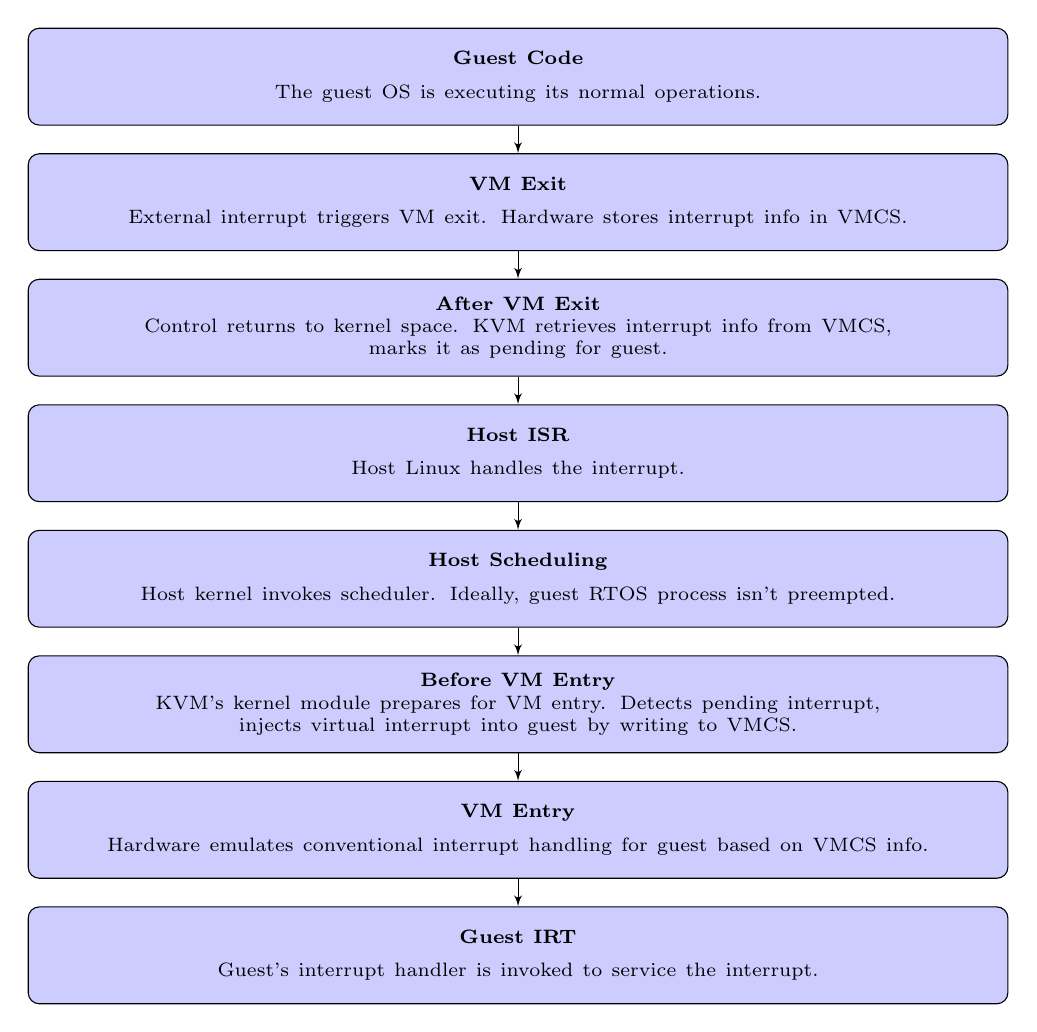
\begin{tikzpicture}[node distance = 0.35cm, auto, % Adjusted node distance
			block/.style={
					rectangle,
					draw,
					fill=blue!20,
					text width=35em,
					rounded corners,
					minimum height=3.5em,
					align=center,
					inner sep=0.2em % Adjusted inner separation
				},
			line/.style={draw, -latex'}
		]
		% Place nodes
		\node [block] (init) {\scriptsize \textbf{Guest Code}\\  The guest OS is executing its normal operations.};
		\node [block, below=of init] (vmexit) {\scriptsize \textbf{VM Exit}\\  External interrupt triggers VM exit. Hardware stores interrupt info in VMCS.};
		\node [block, below=of vmexit] (aftervmexit) {\scriptsize \textbf{After VM Exit}\\  Control returns to kernel space. KVM retrieves interrupt info from VMCS,\\\vspace{-0.5em} marks it as pending for guest.};
		\node [block, below=of aftervmexit] (hostisr) {\scriptsize \textbf{Host ISR}\\  Host Linux handles the interrupt.};
		\node [block, below=of hostisr] (hostscheduling) {\scriptsize \textbf{Host Scheduling}\\  Host kernel invokes scheduler. Ideally, guest RTOS process isn't preempted.};
		\node [block, below=of hostscheduling] (beforevmentry) {\scriptsize \textbf{Before VM Entry}\\  KVM's kernel module prepares for VM entry. Detects pending interrupt,\\\vspace{-0.5em} injects virtual interrupt into guest by writing to VMCS.};
		\node [block, below=of beforevmentry] (vmentry) {\scriptsize \textbf{VM Entry}\\  Hardware emulates conventional interrupt handling for guest based on VMCS info.};
		\node [block, below=of vmentry] (guestirt) {\scriptsize \textbf{Guest IRT}\\  Guest's interrupt handler is invoked to service the interrupt.};
		% Draw edges
		\path [line] (init) -- (vmexit);
		\path [line] (vmexit) -- (aftervmexit);
		\path [line] (aftervmexit) -- (hostisr);
		\path [line] (hostisr) -- (hostscheduling);
		\path [line] (hostscheduling) -- (beforevmentry);
		\path [line] (beforevmentry) -- (vmentry);
		\path [line] (vmentry) -- (guestirt);
	\end{tikzpicture}
	\caption{Flowchart of operations in a virtualized environment}
	\label{fig:kvm_stages}
\end{figure}

\noindent The paper also details several performance tuning methods, including CPU shielding and prioritization, which have been applied in this work.

\bigskip \noindent \citeauthor{broskyShieldedProcessorsGuaranteeing2003} \cite{broskyShieldedProcessorsGuaranteeing2003} report in their work about the shielded CPU model for enhancing real-time performance in symmetric multiprocessor systems. By dedicating one or more CPUs to high-priority processes and interrupts, the goal is to provide deterministic execution of real-time applications and interrupt responses. The authors mention that there is no user interface for setting process CPU affinity in the standard Linux, while there is one for setting interrupt CPU affinity via the \texttt{/proc/irq/*/smp\_affinity} files. These files were used in this masther's thesis. According to the authors, the shielded CPU model is especially useful for tasks that require guaranteed interrupt response times, very fast interrupt responses and high-frequency, deterministic execution.

\bigskip \noindent \citeauthor{kiszkaLinuxRealTimeHypervisor} \cite{kiszkaLinuxRealTimeHypervisor} specifically focuses on Linux as a hypervisor and analyzes its real-time capabilities when using KVM and QEMU. Most importantly for this master's thesis, the author warns of starvation when the priorities of QEMU’s threads are raised and lifted into a real-time scheduling class. Starvation is when a process does not get the resources it needs for a long time because the resources are being allocated to other processes. A way to reduce this risk is by not using more virtual CPUs (VCPUs) than there are actual processor cores. Moreover, Linux has a feature that can limit how much CPU time all real-time tasks can use in the host system, which was an important information for the real-time tunings of this thesis later.

\bigskip \noindent \citeauthor{mckenneyRealTimeVs} \cite{mckenneyRealTimeVs} addresses the overheads associated with real-time Linux when using KVM and QEMU. The author lists several sources of overhead, including memory locking to avoid page-fault latencies, increased overhead of locking and interrupts due to more-aggressive preemption, threaded interrupts that permit long-running interrupt handlers to be preempted by high-priority real-time processes, real-time task scheduling that requires global scheduling, high-resolution timers for tens-of-microseconds accuracy and precision, and preemptible RCU which has slightly higher read-side overhead than Classic RCU. These information helped understand the trade-offs involved in real-time Linux systems.

\bigskip \noindent \citeauthor{deoliveiraDemystifyingRealTimeLinux} \cite{deoliveiraDemystifyingRealTimeLinux} critique the traditional \texttt{cyclictest} tool used for measuring scheduling latency, highlighting its limitations due to its black-box approach and lack of theoretical grounding. This is the main reason why this tool was not used to measure the scheduling latency in this work. Instead, the \texttt{latency} tool was used, as was determined in Chapter \ref{sec:application_context}.


\bigskip \noindent \textcolor{red}{Asymmetric Scheduling and Load Balancing for Real-Time on Linux SMP
	Authors: Eric Piel, Philippe Marquet, Julien Soula, and Jean-Luc Dekeyser12
	The paper presents ARTiS, a real-time extension of the GNU/Linux scheduler designed for SMP (Symmetric Multi-Processors) systems3. ARTiS aims to guarantee the preemption of processors for real-time tasks by assigning specific processors to these tasks4. This system ensures low latency by migrating non-preemptible tasks away from real-time processors5. ARTiS also incorporates load-balancing strategies to fully utilize SMP systems without wasting resources. The implementation of ARTiS involves modifications to the Linux scheduler, resulting in significant improvements in latency compared to the standard Linux scheduler6. The paper details the performance evaluation of ARTiS, highlighting its ability to maintain low interrupt latency even under high system load, making it suitable for hard real-time applications. The authors propose further enhancements, including the integration of real-time scheduling policies like EDF (Earliest Deadline First) and RM (Rate Monotonic)7.}

\bigskip \noindent \textcolor{red}{Title: A Comprehensive Study of Kernel (Issues and Concepts) in Different Operating Systems12
	Authors: Hayfaa Subhi Malallah, Subhi R. M. Zeebaree, Rizgar R. Zebari, Mohammed A. M. Sadeeq, Zainab Salih Ageed, Ibrahim Mahmood Ibrahim, Hajar Maseeh Yasin, Karwan Jameel Merceedi
	Summary: This paper provides an in-depth comparative analysis of various operating systems (OS) focusing on their kernels, which are the core components managing system resources and providing essential services. The study examines the strengths and limitations of popular OS such as iOS, Android, Mac, Windows, and Linux3. It highlights that Linux, Android, and Windows 10 are particularly noted for their stability, compatibility, and reliability4. The paper discusses the evolution of OS kernels, including microkernels, monolithic kernels, and hybrid kernels, and their respective advantages and challenges. It also addresses modern developments in OS technology, such as multicore processors, cloud computing, and the Internet of Things (IoT), and their impact on kernel design and performance. The authors emphasize the importance of security in kernel development, noting that vulnerabilities can lead to significant system compromises. The paper concludes with a discussion on the future directions of OS kernel research and development, advocating for continuous improvement in performance, security, and adaptability to emerging technologies.}

\bigskip \noindent \textcolor{red}{Title: Testing the limits of general-purpose hypervisors for real-time control systems
	Authors: Rui Queiroz, Tiago J. Cruz, Paulo Simões (University of Coimbra)
	Summary: This paper explores the feasibility of using general-purpose off-the-shelf hypervisors to virtualize real-time control systems within the context of Industry 4.0. The authors address the need for flexibility, security, and resilience in automation infrastructures while maintaining real-time requirements. They discuss the potential benefits of virtualizing servers and control devices in Industrial and Automation Control Systems (IACS), but also highlight the challenges due to the focus of general-purpose hypervisors on maximizing throughput, often at the expense of determinism and increased latency.
	The paper presents an empirical evaluation of various hypervisors, concluding that while some are capable of handling typical real-time workloads, this capability cannot be generalized to all types of real-time systems. The authors provide a comprehensive analysis of cyber-physical systems (CPS), control devices, and real-time systems, including their latency and jitter requirements. They also delve into the specifics of real-time operating systems (RTOS) and mixed-criticality systems, and review different virtualization techniques, comparing commercial off-the-shelf hypervisors with real-time hypervisors.
	The study emphasizes the importance of ensuring both spatial and temporal isolation in virtualized environments to maintain predictable real-time performance. It also discusses the role of scheduling policies in real-time applications and the challenges of I/O sharing between multiple virtual machines. The authors conclude that while general-purpose hypervisors show promise, further research and development are needed to fully realize their potential in real-time control systems.}

\bigskip \noindent \textcolor{red}{“Testing the limits of general-purpose hypervisors for real-time control systems” by Rui Queiroz, Tiago J. Cruz, and Paulo Simões from the University of Coimbra:
	With the advent of Industry 4.0, there is a growing need for flexibility, security, and resilience in industrial automation infrastructures while maintaining real-time requirements. This paper explores the feasibility of using general-purpose off-the-shelf hypervisors to virtualize cyber-physical systems’ servers and control devices. The authors, Rui Queiroz, Tiago J. Cruz, and Paulo Simões, present an empirical evaluation of these hypervisors, focusing on their ability to handle real-time workloads. The study highlights the challenges posed by the need for determinism and low latency, which are often compromised by hypervisors designed to maximize throughput. The paper concludes that while some hypervisors can manage typical real-time workloads, this capability is not universal across all types of real-time systems. The research underscores the importance of understanding the limits and capabilities of conventional hypervisors to ensure they meet the specific requirements of industrial automation control systems.}

\bigskip \noindent \textcolor{red}{Title: A State-of-the-Art Survey on Real-Time Issues in Embedded Systems Virtualization
	Authors: Zonghua Gu and Qingling Zhao
	Summary: This paper provides a comprehensive survey on real-time issues in virtualization for embedded systems, authored by Zonghua Gu and Qingling Zhao. Virtualization, widely accepted in server and cloud computing, has been increasingly applied to embedded systems with stringent timing constraints. The paper discusses various virtualization systems, including KVM, Xen, and L4, and their applications in embedded systems such as avionics, industrial automation, and mobile phones. It highlights the importance of real-time performance, security, and dependability in these systems. The survey covers different types of virtualization, including Type-1 (bare-metal) and Type-2 (hosted) virtualization, as well as full and para-virtualization. It also addresses specific real-time issues like scheduling, partitioning, and the Lock-Holder Preemption problem. The paper concludes with a discussion on the future directions and challenges in the field of real-time virtualization for embedded systems.}

\bigskip \noindent \textcolor{red}{Impact of Modern Virtualization Methods on Timing Precision and Performance of High-Speed Applications
	Authors: Veronika Kirova, Kirill Karpov, Eduard Siemens, Irina Zander, Oksana Vasylenko, Dmitry Kachan, Sergii Maksymov
	This research investigates the precision of timing methods and their efficiency in various virtual environments, focusing on their impact on high-speed network applications. The study examines how timer hardware is shared among CPU- and I/O-bound tasks on both virtualized and bare operating systems. By replacing timing methods within an application for estimating available path bandwidth, the authors analyze the impact on estimation accuracy. The findings highlight that timer overhead and precision are crucial for high-performance network applications, with low-precision timing methods leading to degradation in virtual environments. The paper confirms that using precise timing operations and AvB estimation methods can overcome inefficiencies in standard time-related operations. The research evaluates five different virtual environments to determine the most optimal for high-speed network applications, providing a comprehensive analysis of the impact of virtualization on timing precision and performance.}

\bigskip \noindent \textcolor{red}{“Real Time Operating Systems: A Complete Overview” by Mrinal Parikshit Chandane:
	The paper “Real Time Operating Systems: A Complete Overview” by Mrinal Parikshit Chandane provides an in-depth examination of Real Time Operating Systems (RTOS) and their critical role in embedded systems, particularly in telecommunication applications such as telephony, navigation, and military signaling systems. RTOS is essential for applications that require strict deadline constraints and the ability to handle multiple tasks simultaneously1. The paper highlights the key features of RTOS, including timing considerations, task prioritization, and communication and synchronization between tasks2.
	The document delves into various design aspects necessary for developing an RTOS, such as task management, multitasking, context switching, task priority, and kernel functions3. It explains how tasks are created, prioritized, and managed within an RTOS, emphasizing the importance of efficient CPU utilization and the prevention of data corruption through mutual exclusion. The paper also discusses the implementation of RTOS, covering topics like programming language selection, task stack management, and the initialization process.
	Furthermore, the paper presents a practical example of designing and implementing an RTOS for a Philips 8052 microcontroller, demonstrating the application of theoretical concepts in real-world scenarios. The successful implementation of applications such as a column controller, digital calculator, and dancing LEDs showcases the versatility and effectiveness of RTOS in managing complex embedded systems4.
	Overall, the paper provides a comprehensive overview of RTOS, offering valuable insights into its architecture, design, and implementation, making it a significant contribution to the field of embedded systems5.}

\bigskip \noindent \textcolor{red}{The paper “Challenges in Real-Time Virtualization and Predictable Cloud Computing” explores the integration of real-time systems with cloud computing and virtualization technologies. The authors, Marisol García-Valls, Tommaso Cucinotta, and Chenyang Lu, identify the significant technical challenges in supporting real-time applications within cloud environments1. They highlight that while cloud computing offers benefits such as reduced operational costs, server consolidation, and elastic resource provisioning, it struggles to meet the demands of soft real-time applications like online video streaming, cloud-based gaming, and telecommunication management2. These applications require predictable performance in open, shared, and virtualized environments3.
	The paper discusses the evolution of cloud computing, emphasizing the shift from local computing resources to distributed cloud-based models. It outlines the benefits of virtualization, including functional execution isolation, easier management, and the coexistence of legacy and new applications4. However, the authors note that the multi-tenant nature of cloud computing introduces challenges in providing stable and predictable performance due to resource sharing among multiple virtual machines (VMs).
	The authors delve into various virtualization techniques, such as full virtualization, hardware-assisted virtualization, para-virtualization, OS-level virtualization, and application-level virtualization, each with its performance characteristics and suitability for real-time applications. They also address the importance of real-time scheduling and resource management in virtualized environments, highlighting the need for hierarchical scheduling and the role of real-time hypervisors.
	The paper concludes by presenting potential future research directions to enhance the predictability and performance of cloud-based real-time applications, emphasizing the need for improved resource management frameworks and real-time virtualization techniques.}

\bigskip \noindent \textcolor{red}{The paper titled “VM-Based Real-Time Services for Automotive Control Applications” is authored by Alejandro Masrur, Sebastian Drossler, Thomas Pfeuffer, and Samarjit Chakraborty. It explores the use of Virtual Machines (VMs) to provide real-time services in automotive control applications12. The authors utilize the Xen hypervisor to design a real-time control loop on top of a virtualization layer3. They first analyze a typical Xen configuration and identify issues when used for real-time applications4. The paper highlights that the SEDF (Simple Earliest Deadline First) scheduler in Xen can be improved with minimal modifications to enhance worst-case performance5. To further reduce latency and jitter, the authors propose a new scheduler for Xen that prioritizes real-time VMs using a fixed-priority policy6. This approach ensures that timing constraints in automotive control applications are met7. The paper includes extensive experiments to illustrate the effectiveness of the proposed solutions.}

\bigskip \noindent \textcolor{red}{Title: Hard Real Time Linux* Using Xenomai* on Intel® Multi-Core Processors12
	Author: Amarpreet Singh Ugal, BIOS/Firmware Engineer, Intel Corporation
	Summary: This document explores the implementation of hard real-time capabilities in Linux using Xenomai on Intel® multi-core processors. Traditional Linux is not a hard real-time operating system because it cannot guarantee that tasks will meet strict deadlines34. To address this, the document discusses the use of a high-priority real-time kernel that runs between the hardware and standard Linux. This real-time kernel executes real-time tasks and suspends normal Linux processes during this period56. The real-time scheduler treats the standard Linux kernel as an idle task, allowing real-time tasks to preempt normal processes78. Xenomai, which uses an interrupt pipeline from the ADEOS project, is highlighted as a solution for managing interrupts and ensuring minimal latency and jitter. The document also covers the installation and configuration of Xenomai on CentOS 5.2, including kernel patching and testing with various tools like switchbench, switchtest, cyclictest, clocktest, and latency. The detailed steps and configurations provided aim to help developers achieve hard real-time performance on Intel® Core™ i7 multi-core processors.}

\bigskip \noindent \textcolor{red}{Title: Performance Assessment of Linux Kernels with PREEMPT\_RT on ARM-Based Embedded Devices
	Authors: George K. Adam, Nikos Petrellis, Lambros T. Doulos
	Summary: This research investigates the real-time performance of Linux kernels and distributions with the PREEMPT\_RT real-time patch on ARM-based embedded devices, specifically BeagleBoard and Raspberry Pi. The study aims to provide novel insights into Linux real-time performance by evaluating various metrics such as response latency, periodic task execution, and maximum sustained frequency using heuristic methods and the cyclictest benchmark tool. The authors introduce a new response task model and develop specific software measurement modules to assess the performance.
	The results demonstrate that the PREEMPT\_RT patch significantly improves real-time performance compared to default Linux kernels, particularly in reducing worst-case latencies. This makes ARM-based devices running Linux with PREEMPT\_RT more suitable for time-sensitive embedded control systems. The research also highlights the growing use of Linux in embedded systems for real-time applications, driven by its open-source nature, performance, and adaptability to various hardware systems. The methodology and findings of this study could be applied to other Linux-based real-time platforms, contributing to the broader field of real-time systems research.}

\bigskip \noindent \textcolor{red}{Title: Real-Time I/O System for Many-core Embedded Systems 1 Author: Zhe Jiang
	In this thesis, Zhe Jiang addresses the critical need for time predictability in modern real-time embedded systems, particularly focusing on I/O operations. The proposed solution, BlueIO, is a hardware-implemented real-time I/O virtualization system designed to meet the requirements of predictability, timing accuracy, enhanced performance, scalability, parallel access, and isolation simultaneously2. BlueIO integrates key functionalities of I/O virtualization and low-layer I/O drivers through the Virtualized Complicated Device Controller (VCDC) and a clock cycle-level timing-accurate I/O controller, the GPIO Command Processor (GPIOCP)3. This system supports abstract virtualized access to I/O devices from the software domain, providing isolation and concurrent access to I/O operations, thereby improving performance45. The thesis also introduces BlueVisor, a scalable real-time hardware hypervisor built upon BlueIO, enabling predictable virtualization on CPU, memory, and I/O, along with fast interrupt handling and inter-virtual machine communication67. The work demonstrates significant improvements in I/O performance and low running costs across different operating systems, with a hardware consumption analysis showing linear scalability with the number of CPUs and I/O devices.}

\bigskip \noindent \textcolor{red}{Title: Real-Time Operating Systems1
	Author: Jiacun Wang, Monmouth University
	Summary: This chapter provides an in-depth overview of Real-Time Operating Systems (RTOS), which are crucial for embedded systems requiring timely and predictable responses. The chapter begins by outlining the main functions of general-purpose operating systems, such as process management, memory management, interrupts management, multitasking, file system management, and I/O management. It then delves into the specific characteristics of RTOS kernels, emphasizing the need for predictable timing behavior, priority scheduling, intertask communication, and resource sharing. The chapter also discusses clocks and timers, asynchronous I/O, and memory locking as essential features of RTOS. Finally, it provides examples of widely used RTOS products, including LynxOS, OSE, QNX, VxWorks, and Windows Embedded Compact, highlighting their unique features and applications in various industries such as aerospace, automotive, and telecommunications.}

\bigskip \noindent \textcolor{red}{Title: Real-Time Scheduling: From Hard to Soft Real-Time Systems1
	Authors: Giuseppe Lipari (Université de Lille) and Luigi Palopoli (Università di Trento)
	Summary: This paper explores the evolution of real-time systems, traditionally divided into hard real-time and soft real-time categoriesHard real-time systems are critical, where missing a deadline can lead to catastrophic consequences, such as in automotive brake systems2. Soft real-time systems, on the other hand, aim to optimize the quality of service, like multimedia players that can tolerate occasional delays without severe impact.
	The authors argue that the boundary between these two categories is becoming increasingly blurred. They introduce the concept of time-predictability and criticality to understand the origins of real-time deadlines. The paper presents the resource reservation framework as a method for scheduling both hard and soft real-time tasks. This framework enhances system robustness and resource utilization by isolating the temporal behavior of tasks.
	The paper also discusses the Constant Bandwidth Server (CBS) algorithm, which integrates with the EDF scheduler to manage execution budgets and periods, ensuring temporal isolation3. The authors highlight the importance of designing systems that remain consistent even when deadlines are missed, emphasizing the need for robust software development practices.
	In conclusion, the paper demonstrates how resource reservation techniques can be applied to classical control systems, improving performance and robustness4. The authors provide a comprehensive overview of existing techniques and tools for soft real-time scheduling and analysis, making a strong case for the integration of these methods in modern real-time systems5.}

\bigskip \noindent \textcolor{red}{The paper titled “Performance analysis of real-time and general-purpose operating systems for path planning of the multi-robot systems” by Seçkin Canbaz and Gökhan Erdemir explores the performance differences between real-time operating systems (RTOS) and general-purpose operating systems (GPOS) in the context of multi-robot systems. The study focuses on two Linux distributions, Ubuntu and Pardus, and evaluates their effectiveness as both GPOS and RTOS for path planning tasks12. The authors highlight the critical distinction between GPOS and RTOS, emphasizing that RTOS can preempt low-priority tasks with high-priority ones, even during kernel calls, which is not possible in GPOS.
	The research involves using the turtlesim simulation environment to perform path tracking tasks with robot groups of varying sizes. The experiments compare CPU usage and processing times across the different operating systems. Results indicate that Ubuntu GPOS generally outperforms other configurations in terms of lower CPU usage and shorter processing times3. However, RTOS configurations, while slower, offer higher system security and reduced error margins due to their strict time management.
	The study concludes that while GPOS may be preferable for performance-centric applications, RTOS is essential for tasks with high time dependency. The authors suggest that the choice between GPOS and RTOS should consider factors such as potential failure conditions, process security, and processing time requirements. This research provides valuable insights into the suitability of different operating systems for multi-robot applications, contributing to the broader field of robotics and autonomous systems.}

\bigskip \noindent \textcolor{red}{Title: The Real-Time Linux Kernel: A Survey on PREEMPT\_RT12
	Authors: Federico Reghenzani, Giuseppe Massari, and William Fornaciari from Politecnico di Milano3
	Summary: This survey explores the evolution and current state of the PREEMPT\_RT patch for the Linux kernel, which aims to enhance the real-time capabilities of Linux. The authors discuss the increasing demand for real-time applications and the challenges posed by using Commercial-Off-The-Shelf (COTS) hardware in such environments. The PREEMPT\_RT patch modifies the existing Linux kernel to improve predictability and reduce latencies, making it suitable for real-time applications. The survey covers various approaches to real-time Linux, including cokernel approaches like RTLinux, Xenomai, and RTAI, and compares them with the PREEMPT\_RT patch4. The authors highlight the benefits of using Linux in real-time systems, such as the availability of rich hardware support and a well-established programming environment. They also discuss the challenges of integrating real-time capabilities into a general-purpose operating system and the ongoing efforts to address these issues. The survey concludes with an overview of industrial and scientific use cases that have benefited from the PREEMPT\_RT patch, emphasizing its significance in fields like aerospace, automotive, and high-performance computing.}


\bigskip \noindent \textcolor{red}{The paper titled “Performance Evaluation of Xenomai 3” by Ching-Chun (Jim) Huang, Chan-Hsiang Lin, and Che-Kang Wu, presents an in-depth analysis of Xenomai 3, a real-time framework for Linux. Xenomai 3 operates either as a dual-kernel system alongside Linux or natively over mainline Linux kernels, enhanced by PREEMPT RT for stricter response times1. The study evaluates Xenomai 3’s performance, particularly in dual-kernel configuration, using ARM Cortex-A series benchmarks. The authors highlight Xenomai 3’s optimizations in RTOS API emulation, thread-to-thread communications, and reduced overhead. The paper compares Xenomai 3 with its predecessor, Xenomai 2, and the PREEMPT RT-enhanced Linux kernel, demonstrating superior maximum response times to external interrupts in dual-kernel setups. The study employs BeagleBone Black hardware and various kernel configurations to measure latencies under idle and CPU-stressed conditions2. Results indicate that Xenomai 3 generally outperforms Xenomai 2 and PREEMPT RT, except for a slight degradation in timer-IRQ latency under stress. The paper concludes that Xenomai 3 offers significant improvements in real-time performance and flexibility, making it a robust choice for real-time applications.}


\section{Problem and Task Definition}



\section{Objective}

The main objective of this work is to create a real-time robot control platform that integrates Salamander OS, Xenomai, QEMU and PCV-522 in the Yocto environment.


\clearpage


\chapter{Theoretical Foundations}
\section{Yocto}\label{sec:yocto}

\section{QEMU}\label{sec:qemu}

\section{Xenomai}\label{sec:xenomai}
\noindent Xenomai 3~\cite{XenomaiXenomai} is an open-source real-time framework that offers two paths to real-time performance. The first approach supplements the Linux kernel with a compact real-time core dubbed Cobalt, demonstrated in Figure~\ref{fig:cobalt}. Cobalt runs side-by-side with Linux, but it handles all time-critical activities like interrupt processing and real-time thread scheduling with higher priority than the regular kernel activities.

\begin{figure}[H]
	\centering
	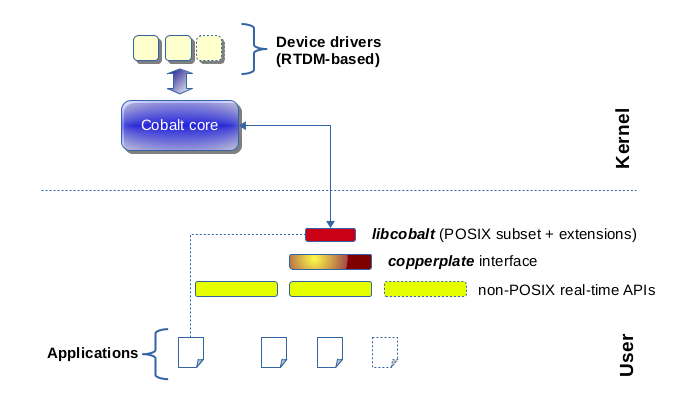
\includegraphics[width=0.8\columnwidth]{img/introduction/xenomai/x3-cobalt-interfaces.png}
	\caption[Xenomai Cobalt interfaces]{Xenomai Cobalt interfaces~\cite{XenomaiXenomai}}
	\label{fig:cobalt}
\end{figure}

\noindent  The second approach, called Mercury and shown in Figure~\ref{fig:mercury}, relies on the real-time capabilities already present in the native Linux kernel. Often, applications require the PREEMPT-RT extension to augment the mainline kernel's real-time responsiveness and minimize jitter, but this isn't mandatory and depends on the application's specific requirements for responsiveness and tolerance for occasional deadline misses.


\begin{figure}[H]
	\centering
	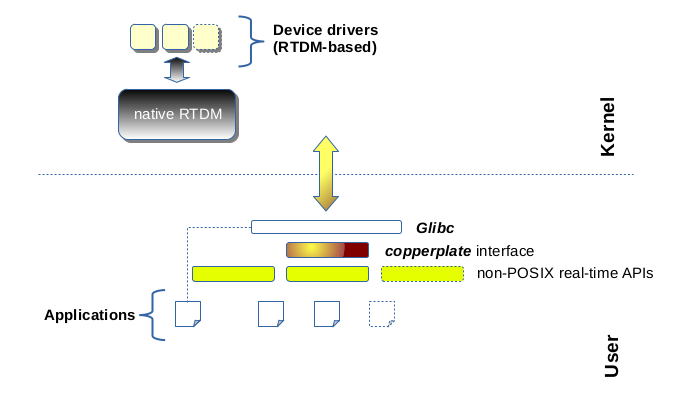
\includegraphics[width=0.8\columnwidth]{img/introduction/xenomai/x3-mercury-interfaces.png}
	\caption[Xenomai Mercury interfaces]{Xenomai Mercury interfaces~\cite{XenomaiXenomai}}
	\label{fig:mercury}
\end{figure}

\noindent Salamander 4 uses the Cobalt real-time core with the Dovetail extension, which allows the kernel to handle real-time tasks with low latency.

\section{VARAN-Bus}\label{sec:varan}

\section{Salamander 4}\label{cha:salamander4}
This chapter briefly describes the Salamander 4 operating system by SIGMATEK.

\subsection{Structure}
\noindent Salamander 4 is the proprietary operating system of SIGMATEK. It is based on Linux version 5.15.94 and integrates Xenomai 3.2, a real-time development environment~\cite{XenomaiXenomai}. Salamander 4 is a 64-bit system, which refers to the x86\_64 architecture. The real-time behaviour is achieved through the use of Symmetric Multi-Processing (SMP) and Preemptive Scheduling (PREEMPT). In addition, it uses IRQPIPE to process interrupts in a way that meets the real-time requirements of the system. The output of the command~\texttt{uname -a} can be observed in code~\ref{output:uname_a_virt}.

\vspace{1em}
\begin{minipage}{0.95\columnwidth}
	\begin{lstlisting}[name={System information},label={output:uname_a_virt}]
root@sigmatek-core2:~# uname -a
Linux sigmatek-core2 5.15.94 #1 SMP PREEMPT IRQPIPE Tue Feb 14 18:18:05 UTC 2023 x86_64 GNU/Linux
\end{lstlisting}
\end{minipage}

\noindent Salamander 4 is powered by SIGMATEK's CP 841~\cite{CPUEinheitenSIGMATEK} and is comprised of the following software modules:

\begin{itemize}
	\item \textbf{Operating system}: The operating system in a LASAL CPU manages the hardware and software resources of the system. It is provided in a completely PC-compatible manner, working with a standard PC BIOS.
	\item \textbf{Loader}: The loader is a part of the operating system that is responsible for loading programs from executables into memory, preparing them for execution and then executing them.
	\item \textbf{Hardware classes}: Hardware classes in LASAL represent the different types of hardware components that can be controlled by the LASAL CPU. They provide a way to organize and manage the hardware components in a modular and reusable manner. The graphical hardware editor in LASAL allows for a true-to-detail simulation of the actual hardware.
	\item \textbf{Application}: Applications are developed using LASAL CLASS 2~\cite{EngineeringToolLASAL}, a solution for automation tasks that supports object-oriented programming and design in compliance with IEC 61131-3.
\end{itemize}

\noindent These modules and the interfaces (indicated by an arrow) between them are shown in Figure~\ref{fig:lasal_cpu}.

\begin{figure}[H]
	\centering
	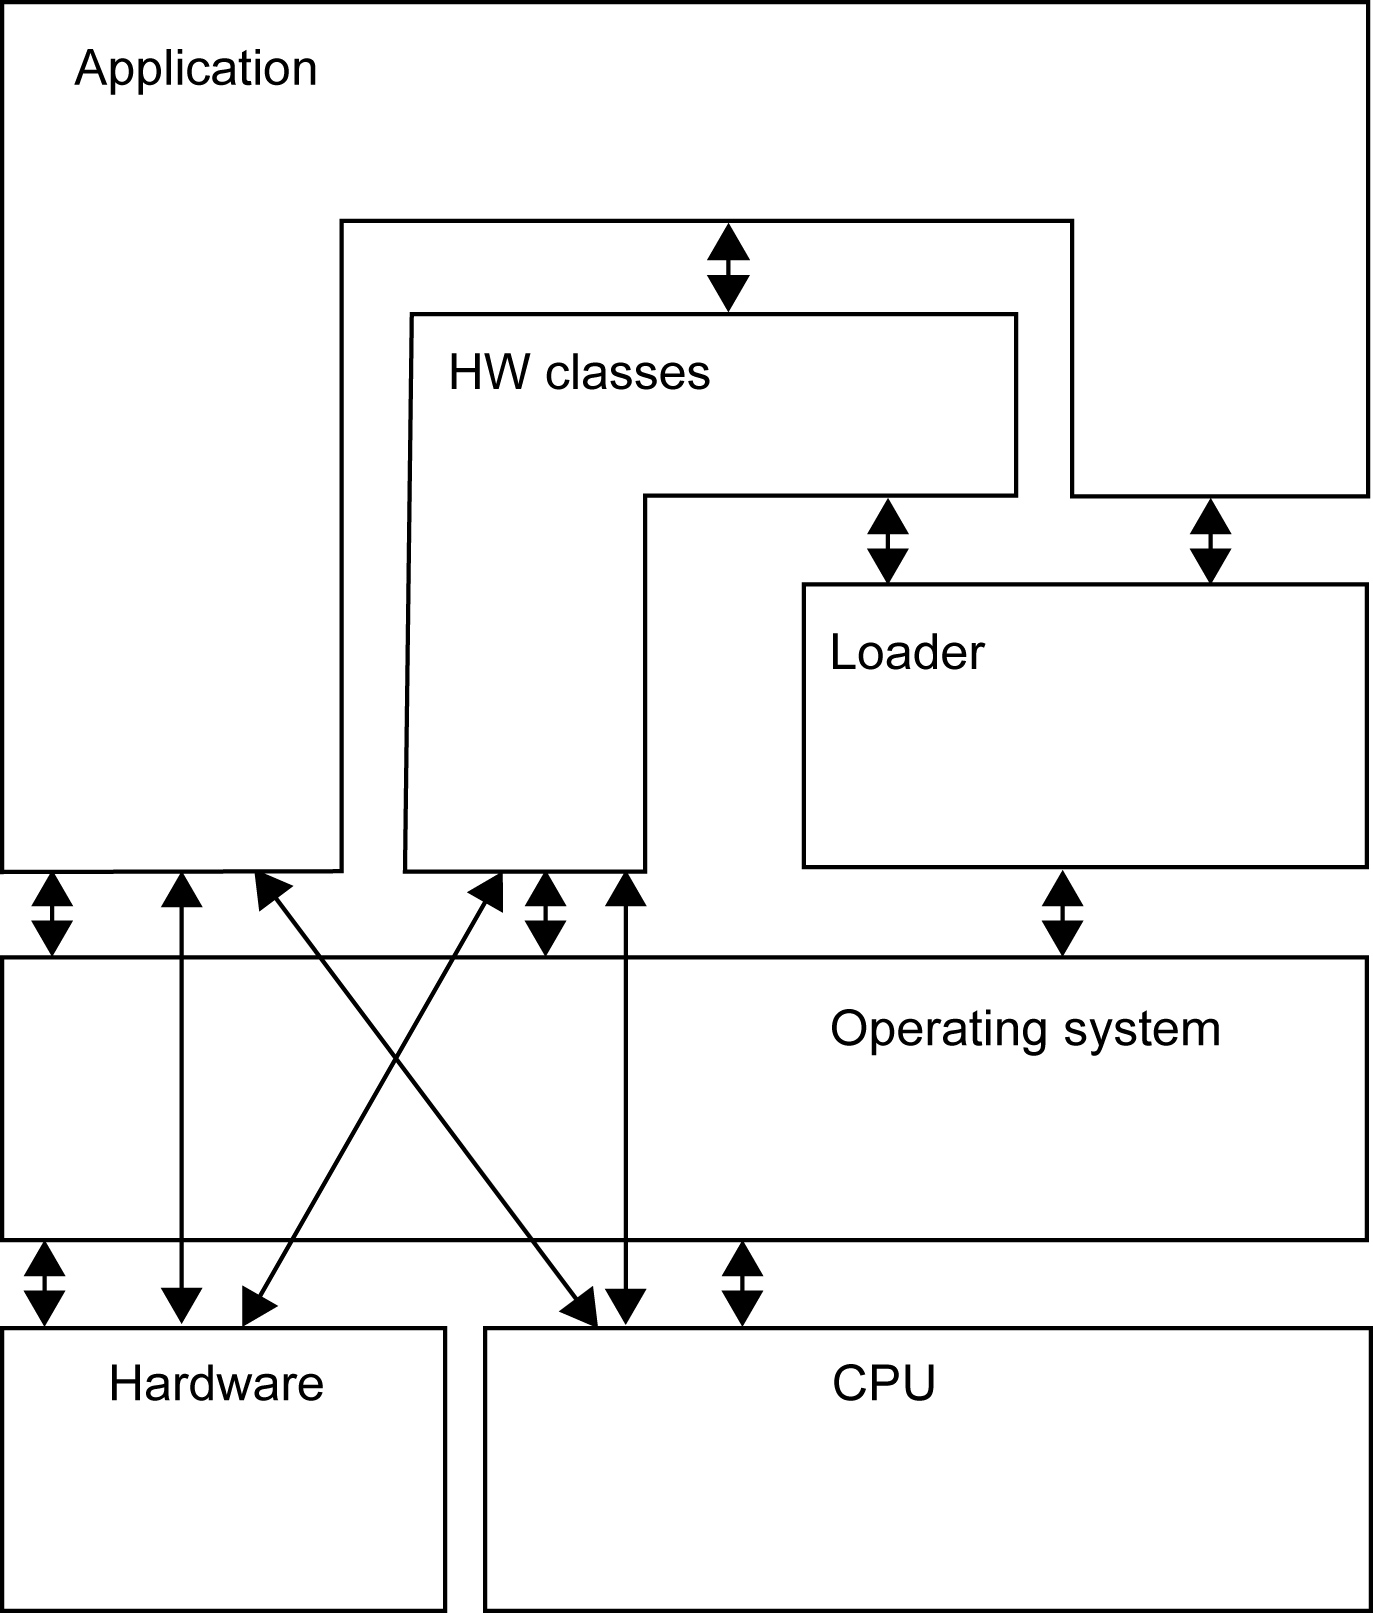
\includegraphics[width=0.5\columnwidth]{img/Software-Struktur_einer_LASAL_CPU.png}
	\caption[Structure of Salamander 4 CPU]{Structure of Salamander 4 CPU}
	\label{fig:lasal_cpu}
\end{figure}

\subsection{Memory Management}
\noindent For the sake of completeness, Figure~\ref{fig:memory_management} displays the memory management of Salamander 4. LRT stands for Lasal Runtime and creates an execution environment where applications developed using the LASAL Class 2 can run, providing defined real-time functions, data types, and other constructs tailored for real-time programming.

\begin{figure}[H]
	\centering
	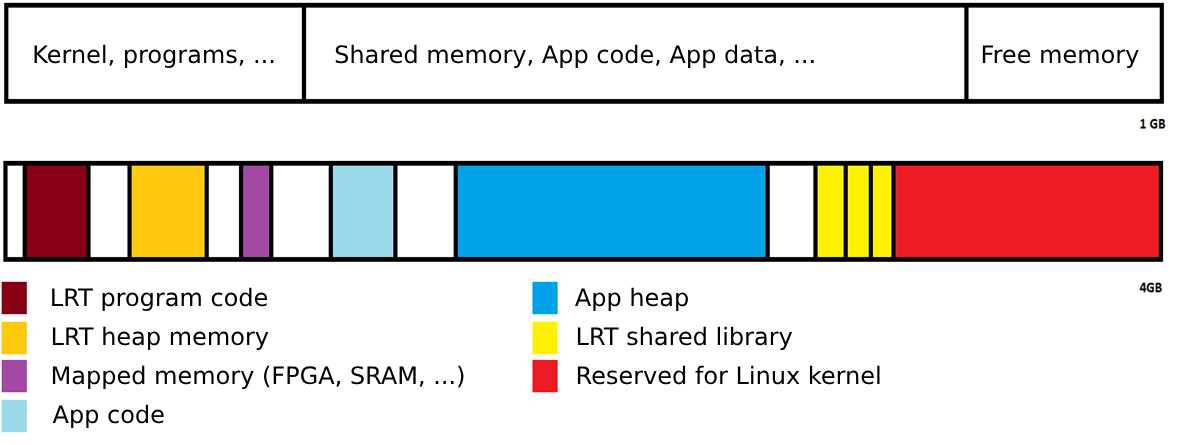
\includegraphics[width=0.8\columnwidth]{img/RAM_Memory_management.png}
	\caption[Memory Management]{Memory Management}
	\label{fig:memory_management}
\end{figure}



\clearpage


\chapter{Methodology}\label{cha:methodology}

This section describes in detail all the theoretical concepts and boundary conditions as well as practical methods that contributed to achieving the objectives of this master's thesis.

\bigskip \noindent Trace-cmd can be used for tracing the Linux kernel~\cite{Tracecmd}. It can record various kernel events such as interrupts, scheduler decisions, file system activity, function calls in real time. Trace-cmd helped in getting detailed insights into system behaviour and identify reasons for latency.

\bigskip \noindent The data that was recorded by trace-cmd was then fed into Kernelshark, which is a graphical front-end tool~\cite{KernelShark}. It visualizes the recorded kernel trace data in a readable way on an interactive timeline, which facilitated the process of identifying patterns and correlations between events. By further filtering the displayed events according to specific criteria such as processes, event types or time ranges, the latency issues were analyzed.

\bigskip \noindent Real-time operating system capabilities were provided by Xenomai, which is real-time development framework that extends the Linux kernel~\cite{XenomaiXenomai}. It enables low-latency and deterministic execution of time-critical tasks. Xenomai 3 introduces a dual-kernel approach with a real-time kernel coexisting alongside Linux. A key utility within the Xenomai suite is the latency tool, which benchmarks the timer latency - the time it takes for the kernel to respond to timer interrupts or task activations. The tool creates real-time tasks or interrupt handlers and measures the latency between expected and actual execution times.

The system configuration is shown in Table~\ref{tab:testbed_configuration}

\begin{table}[H]
	\centering
	\caption[System configuration]{System configuration}
	\label{tab:testbed_configuration}
	\setlength{\tabcolsep}{0.5em} % for the horizontal padding
	{\renewcommand{\arraystretch}{1.2}% for the vertical padding
		\begin{tabular}{|l|l|}
			\hline
			\textbf{CPU}    & 13\textsuperscript{th} Gen Intel(R) Core(TM) i7-13800H \\ \hline
			\textbf{Memory} & 2 $\times$ 16GB SO-DIMM DDR5-5600 MT/s, 32GB           \\ \hline
			\textbf{GPU}    & NVIDIA RTX A500 Laptop GPU                             \\ \hline
			\textbf{BIOS}   & Dell Version 1.12.0                                    \\ \hline
			\textbf{OS}     & Ubuntu 22.04.4 LTS                                     \\
			\hline
		\end{tabular}}
\end{table}

\noindent Figure~\ref{fig:lstopo} is the output of the~\texttt{lstopo} command and visualizes the hardware nodes of the system, including CPU cores, caches, memory, and I/O devices.
\begin{figure}[H]
	\centering
	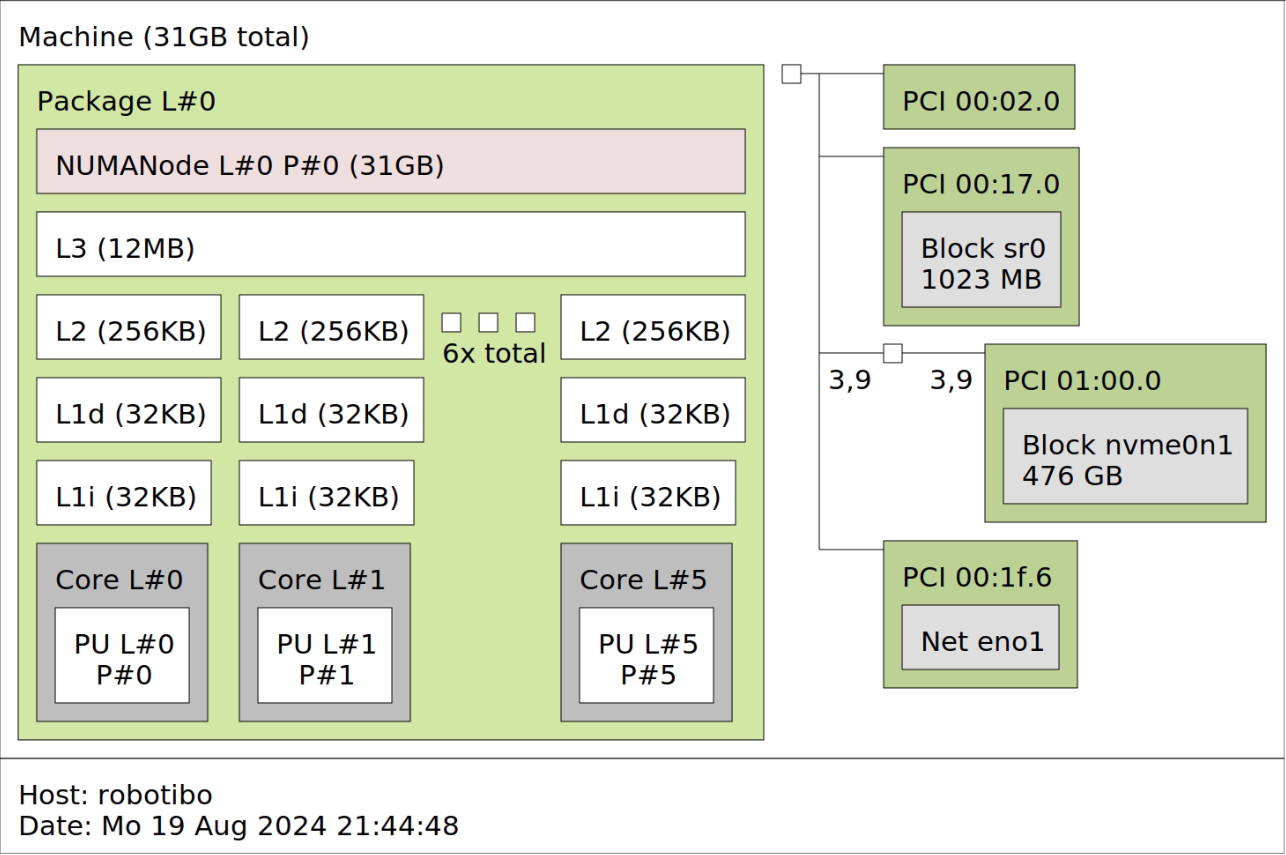
\includegraphics[width=1.0\columnwidth]{img/lstopo.png}
	\caption[Hardware topology]{Hardware topology}
	\label{fig:lstopo}
\end{figure}

\clearpage

\chapter{Initial Real-Time Latency}\label{cha:initial-real-time-latency}

As a starting point, initial latency values of both the bare metal and virtualization versions were measured with the \texttt{latency} tool of the xenomai tool suite. Salamander 4 bare metal refers to the proprietary hardware of SIGMATEK used to employ the custom operating system. Salamander 4 virtualization refers to a virtual version of the Salamander 4 hardware platform, achieved through QEMU/KVM. Sections~\ref{sec:salamander4-bare-metal} and~\ref{sec:salamander4-virtualization} specify the details of the measurements for both versions. In the further course, the aim was to bring the latency values of the virtualization closer to those of the hardware and guarantee deterministic and reliable behavior.

\section{Salamander 4 Bare Metal}\label{sec:salamander4-bare-metal}
The output of the command~\texttt{uname -a} for Salamander 4 bare metal is shown in Code~\ref{output:uname_a_hw}.

\vspace{1em}
\begin{minipage}{0.95\columnwidth}
	\begin{lstlisting}[name={Salamander 4 bare metal system information},label={output:uname_a_hw}]
root@sigmatek-core2:~# uname -a 
Linux sigmatek-core2 5.15.94 #1 SMP PREEMPT IRQPIPE Tue Feb 14 18:18:05 UTC 2023 x86_64 GNU/Linux
\end{lstlisting}
\end{minipage}

\noindent As a reference point, the latency program was executed on Salamander 4 bare metal for a duration of 10 minutes. The complete command used was~\texttt{latency -h -g gnuplot.txt -T 600}, which runs the latency measurement tool for 600 seconds and prints histograms of min, avg, max latencies in a Gnuplot-compatible format to the file~\texttt{gnuplot.txt}. Figure~\ref{fig:max_latency_hardware} shows the gathered latency values in microseconds.

\begin{figure}[H]
	\centering
	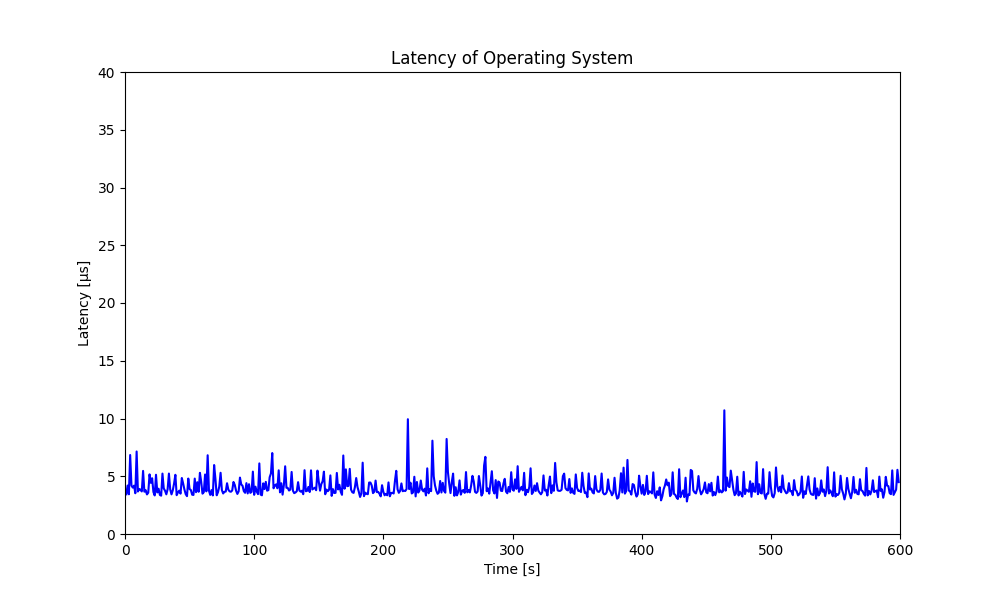
\includegraphics[width=1.0\columnwidth]{img/max_latency_hardware.png}
	\caption[Latency of Salamander 4 bare metal]{Latency of Salamander 4 bare metal}
	\label{fig:max_latency_hardware}
\end{figure}

\noindent The statistics obtained from this measurement are provided in Table~\ref{tab:latency_statistics_bare_metal}. It gives an overview of the average, maximum, minimum latency, and the standard deviation of the latency values in microseconds.


\begin{table}[H]
	\centering
	\caption{Latency statistics of Salamander 4 bare metal in microseconds}
	\label{tab:latency_statistics_bare_metal}
	\setlength{\tabcolsep}{0.5em} % for the horizontal padding
	{\renewcommand{\arraystretch}{1.2}% for the vertical padding
		\begin{tabular}{|c|c|}\hline
			\textbf{Statistic} & \textbf{Value (\textmu s)} \\\hline
			Average Latency    & 4.06                       \\\hline
			Maximum Latency    & 10.71                      \\\hline
			Minimum Latency    & 2.82                       \\\hline
			Standard Deviation & 0.85                       \\\hline
		\end{tabular}}
\end{table}

\noindent Figure~\ref{fig:gnuplot_max_latency_hardware} depicts the variation in latency over the course of said time. Since the data varies strongly, a logarithmic scale was used for both axes.

\begin{figure}[H]
	\centering
	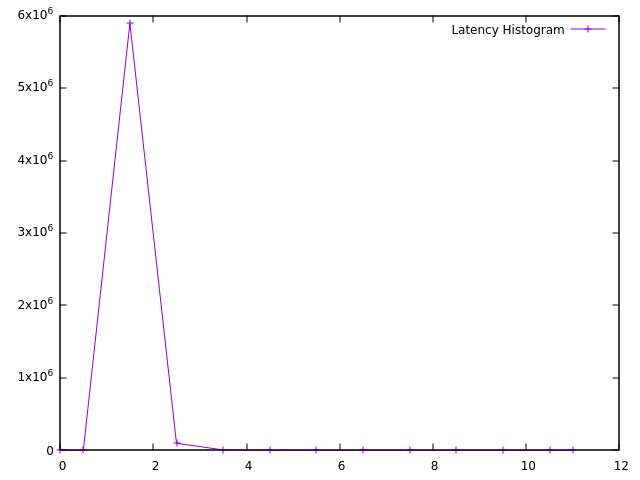
\includegraphics[width=0.7\columnwidth]{masterthesis-documentation/docs/sigmatek/xenomai/0hardware/gnuplot_max_latency_hardware.png}
	\caption[Variation in latency of Salamander 4 bare metal]{Variation in latency of Salamander 4 bare metal}
	\label{fig:gnuplot_max_latency_hardware}
\end{figure}


\section{Salamander 4 Virtualization}\label{sec:salamander4-virtualization}
In addition to providing Salamander 4 on its own hardware, SIGMATEK has also developed a virtualised version of this operating system. It was developed using Yocto, an open-source project that allows customised Linux distributions to be created for embedded systems. Upon generating the necessary files, Yocto provides a QEMU folder with the following components shown in Code~\ref{lst:ls}. QEMU is the environment in which the virtualization runs, as it is an open-source tool for hardware virtualization~\cite{QEMU}.

\vspace{1em}
\begin{minipage}{\linewidth}
	\begin{lstlisting}[name={Contents of QEMU folder for Salamander 4},label={lst:ls}]
    sigma_ibo@localhost:~/Desktop/salamander-image$ ls -1
    bzImage
    drive-c
    ovmf.code.qcow2
    qemu_def.sh
    salamander-image-sigmatek-core2.ext4
    stek-drive-c-image-sigmatek-core2.tar.gz
    vmlinux
    \end{lstlisting}
\end{minipage}

\noindent With the help of the script depicted in Code~\ref{script:qemu_def}, Salamander 4 is started together with the necessary hardware components in the QEMU environment. This makes it possible to run Salamander 4 on a variety of host systems, regardless of the specific hardware of the host. The following is a description of the components used for the virtualization of Salamander 4.
\clearpage
\begin{itemize}
	\item \textbf{bzImage}: Compressed Linux kernel image that is loaded by QEMU at system start. ``bz`` stands for big-zipped.
	\item \textbf{drive-c}: Directory serving as C drive for QEMU system, created and filled by qemu\_def.sh script.
	\item \textbf{ovmf.code.qcow2}: Firmware file for QEMU that enables UEFI boot process. ~\texttt{OVMF} stands for Open Virtual Machine Firmware,~\texttt{qcow2} is a format for disk image files used by QEMU, it stands for ``QEMU Copy On Write version 2''.
	\item \textbf{qemu\_def.sh}: Shell script that starts QEMU with required parameters to boot Salamamder 4 OS. It is described in Code~\ref{script:qemu_def}.
	\item \textbf{salamander-image-sigmatek-core2.ext4}: Disk image of the Salamander 4 OS for the Sigmatek Core 2 platform. It uses the~\texttt{ext4} file system and serves as the root file system in the QEMU virtual machine, acting as the virtual hard drive.
	\item \textbf{stek-drive-c-image-sigmatek-core2.tar.gz}: Compressed tarball containing a pre-configured environment for the Salamander 4 OS. It is unpacked and sets up the~\texttt{drive-c/} directory with system and log files in the~\texttt{qemu\_def.sh} script.
	\item \textbf{vmlinux}: Uncompressed Linux kernel image, typically used for debugging.
\end{itemize}


\begin{comment}
https://www.baeldung.com/linux/kernel-images
\end{comment}


\noindent The inital QEMU script after the custom Yocto build and the starting point for this work is shown in Code~\ref{script:qemu_def}. This script is used to start QEMU with required parameters to boot Salamamder 4 OS. It will be adjusted in Chapter~\ref{cha:real-time_tuning} in order to accompany real-time performance tunings.

\vspace{1em}
\begin{minipage}{\linewidth}
	\begin{lstlisting}[name={QEMU script for starting Salamander 4 virtualization},label={script:qemu_def}]
	#!/bin/sh

	if  [ ! -d drive-c/ ]; then
			echo "Filling drive-c/"
			mkdir drive-c/
			tar -C drive-c/ -xf stek-drive-c-image-sigmatek-core2.tar.gz
	fi
		
	exec qemu-system-x86_64 -M pc,accel=kvm -kernel ./bzImage \
	-m 2048 -drive file=salamander-image-sigmatek-core2.ext4,format=raw,media=disk \
	-append "console=ttyS0 console=tty1 root=/dev/sda rw panic=1 sigmatek_lrt.QEMU=1 ip=dhcp rootfstype=ext4" \
	-net nic,model=e1000,netdev=e1000 -netdev bridge,id=e1000,br=nm-bridge \
	-fsdev local,security_model=none,id=fsdev0,path=drive-c -device virtio-9p-pci,id=fs0,fsdev=fsdev0,mount_tag=/mnt/drive-C \
	-device vhost-vsock-pci,guest-cid=3,id=vsock0 \
	-drive if=pflash,format=qcow2,file=ovmf.code.qcow2 \
	-no-reboot -nographic
\end{lstlisting}
\end{minipage}

\noindent This script is run on a generic Ubuntu 22.04.4 system, as mentioned previously in Chapter~\ref{cha:methodology}. The kernel version and other details are presented in Code~\ref{output:uname_a_ub}, using the~\texttt{uname -a} command.

\vspace{1em}
\begin{minipage}{0.95\columnwidth}
	\begin{lstlisting}[name={Ubuntu 22.04.4 system information},label={output:uname_a_ub}]
root@sigmatek-core2:~# uname -a 
Linux sigma-ibo 6.5.0-35-generic #35~22.04.1-Ubuntu SMP PREEMPT_DYNAMIC Tue May  7 09:00:52 UTC 2 x86_64 x86_64 x86_64 GNU/Linux
\end{lstlisting}
\end{minipage}

\noindent Measuring the latency of the Salamander 4 virtualization with the default QEMU script in Code~\ref{script:qemu_def} and no further adjustments for 10 minutes, the following latency values in Figure~\ref{fig:max_latency_default} were collected.

\begin{figure}[H]
	\centering
	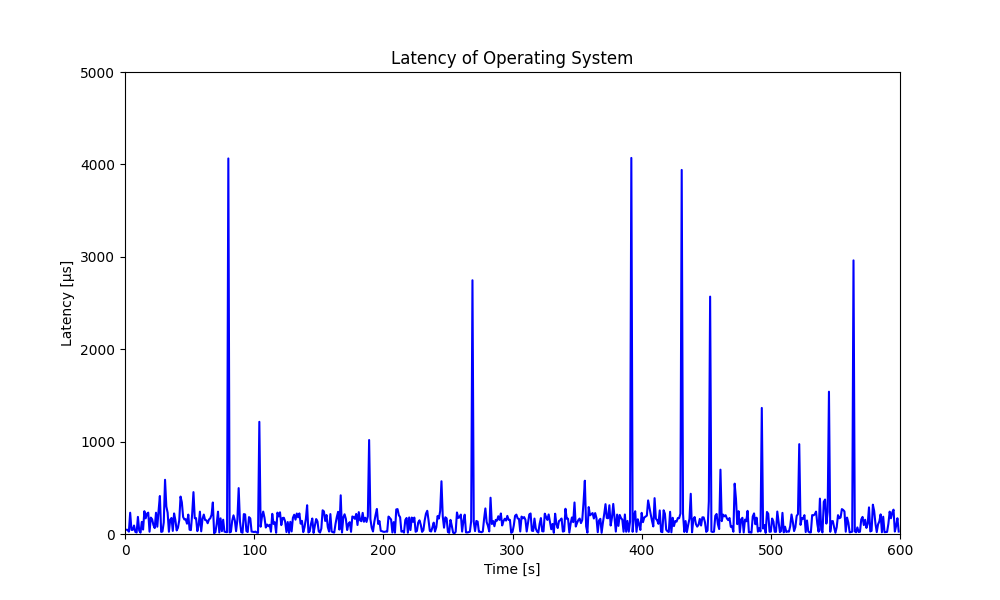
\includegraphics[width=1.0\columnwidth]{img/max_latency_default.png}
	\caption[Latency with default settings]{Latency with default settings}
	\label{fig:max_latency_default}
\end{figure}

\noindent The statistics obtained from this measurement are provided in Table~\ref{tab:latency_statistics_virt}. It gives an overview of the average, maximum, minimum latency, and the standard deviation of the latency values in microseconds.

\begin{table}[H]
	\centering
	\caption{Latency statistics of default Salamander 4 virtualization in microseconds}
	\label{tab:latency_statistics_virt}
	\setlength{\tabcolsep}{0.5em} % for the horizontal padding
	{\renewcommand{\arraystretch}{1.2}% for the vertical padding
		\begin{tabular}{|c|c|}\hline
			\textbf{Statistic} & \textbf{Value (\textmu s)} \\\hline
			Average Latency    & 46.22                      \\\hline
			Maximum Latency    & 707.62                     \\\hline
			Minimum Latency    & 15.59                      \\\hline
			Standard Deviation & 52.13                      \\\hline
		\end{tabular}}
\end{table}

\noindent Figure~\ref{fig:gnuplot_max_latency_default} depicts the variation in latency over the course of said time with default settings.

\begin{figure}[H]
	\centering
	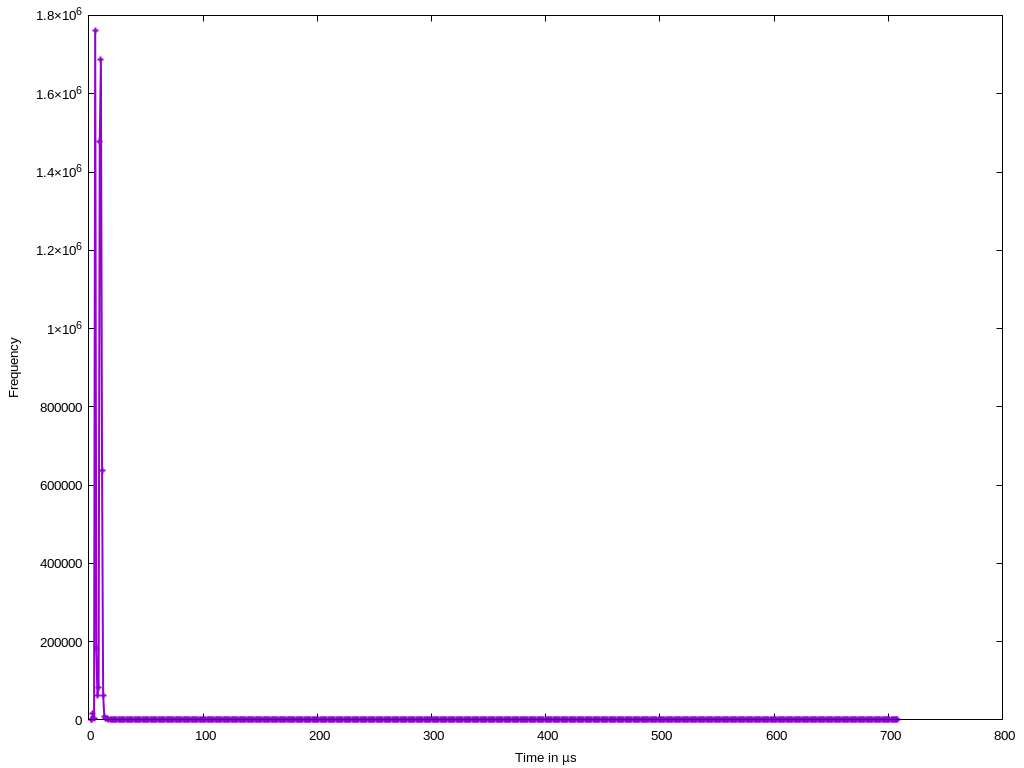
\includegraphics[width=0.7\columnwidth]{masterthesis-documentation/docs/sigmatek/xenomai/1default/gnuplot_max_latency_default.png}
	\caption[Variation in latency with default settings]{Variation in latency with default settings}
	\label{fig:gnuplot_max_latency_default}
\end{figure}


\noindent Comparing these values to those of bare metal in Figure~\ref{fig:gnuplot_max_latency_combined}, it is evident that there is a significant initial gap in the statistics. A maximum latency of 707.62~\textmu s is not tolerable for the system and needs to be tuned.

\begin{figure}[H]
	\centering
	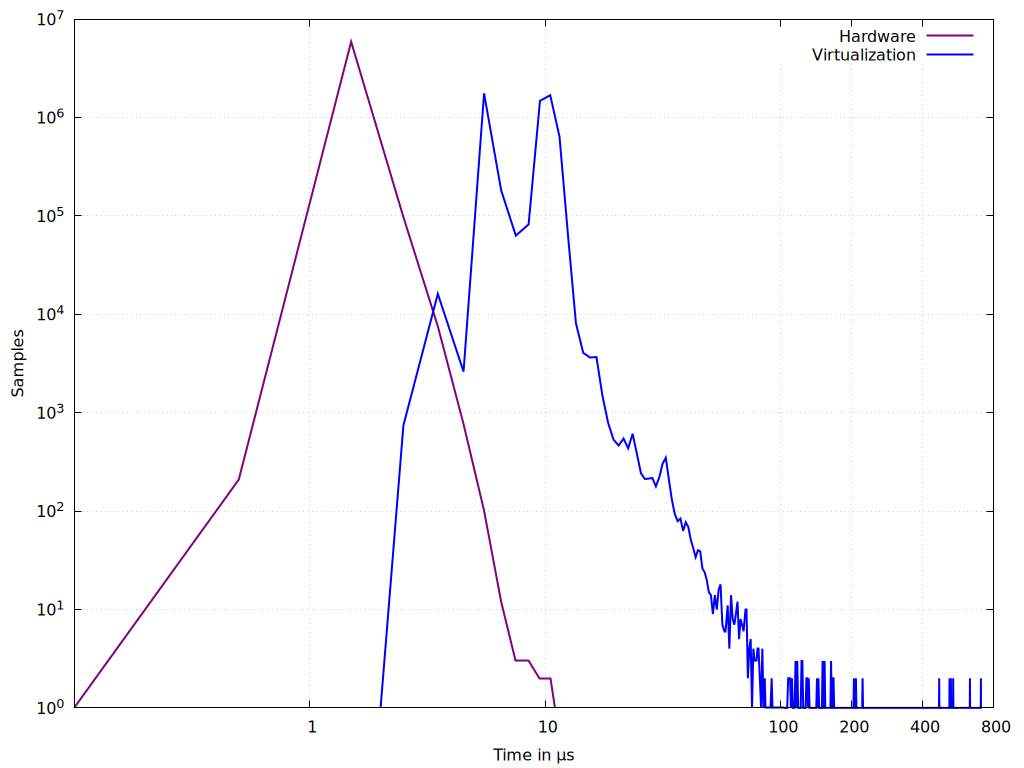
\includegraphics[width=0.7\columnwidth]{masterthesis-documentation/docs/sigmatek/xenomai/01combined/gnuplot_combined_max_latency.png}
	\caption[Comparison of variation in latency between hardware and virtualization]{Comparison of variation in latency between hardware and virtualization}
	\label{fig:gnuplot_max_latency_combined}
\end{figure}



\clearpage

\chapter{Real-Time Performance Tuning}\label{cha:real-time_tuning}

In this chapter, the significant initial gap in latency statistics between the virtualized system and the bare metal system is tackled. For this reason, an extensive tuning process is carried out. This involves configurations spanning the BIOS, kernel, host OS, QEMU/KVM virtualization layer, and the Salamander 4 OS itself. The individual configurations will be discussed in detail and the modifications will be justified with a clear explanation. The goal is to bring the latency of the virtualized system closer to that of the bare metal system, thereby ensuring deterministic behavior under real-time constraints.

\bigskip \noindent It is important to mention that a real-time system implies determinism at every component of the system ranging from hardware over the kernel to the software and the application on it. As already established earlier, the guest OS Salamamder 4 runs Xenomai and is hence real-time capable. The host system also needs to be aware of the real-time determinism in order to achieve highest possible reliability. The very step of achieving the goal of reducing latency is to apply the preempt-rt patch~\cite{RealtimePreempt_rt_versionsWiki} to the host system. This patch is a set of modifications to the Linux kernel with the goal of making it fully preemptible. This means, almost all parts of the kernel can be preempted and higher-priority tasks can interrupt lower-priority ones. This significantly reduces the time it takes for high-priority tasks to start executing after an event~\cite{RealtimeKernelPatchset}. The patch also includes support for high-resolution timers and make the system more predictable, which are crucial for real-time applications where the timing of operations must be guaranteed with precise timing and scheduling~\cite{rostedtInternalsRTPatch}.

\bigskip \noindent Nevertheless, a real-time kernel alone does not make a system truly “real-time”~\cite{WhatRealtimeLinux}. Additional modifications are required to achieve this. The next sections will deal with these real-time performance tunings. The very first step in this regard is the isolation of a CPU to dedicate it solely to the desired real-time task. CPU isolation and affinity will be covered in detail later in Section~\ref{subsec:cpu_isolation}, but its impact will be briefly demonstrated here.


Figure~\ref{fig:max_latency_taskset} shows latency of QEMU taskset Salamander4.
\begin{figure}[H]
	\centering
	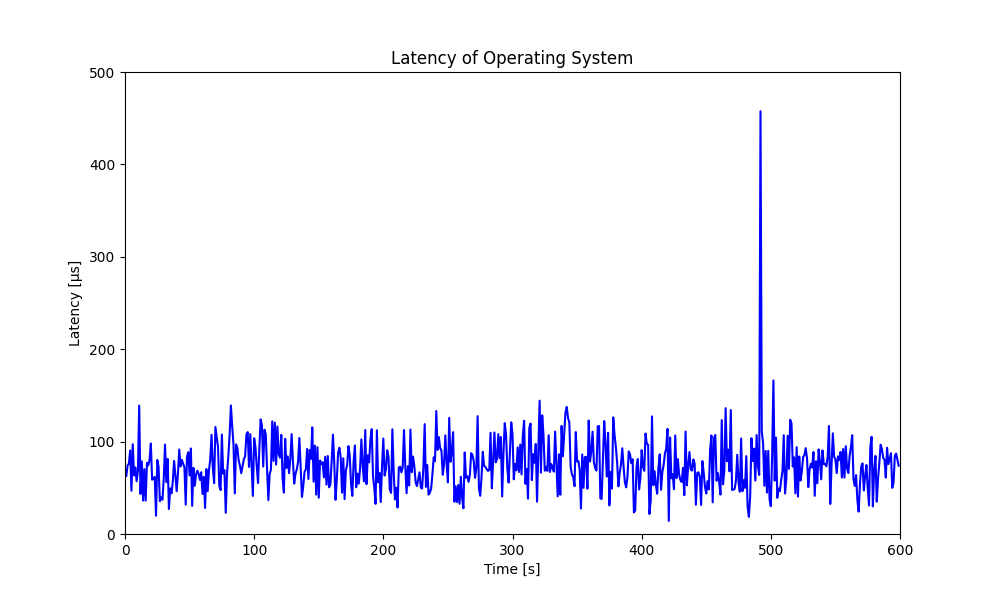
\includegraphics[width=1.0\columnwidth]{img/max_latency_taskset.png}
	\caption[Latency taskset]{Latency taskset}
	\label{fig:max_latency_taskset}
\end{figure}


After each tuning, the latency test of Xenomai will be executed to evaluate the improved latency of the system.

\textcolor{red}{After Article, Figure~\ref{fig:max_latency_rt}}

\begin{figure}[H]
	\centering
	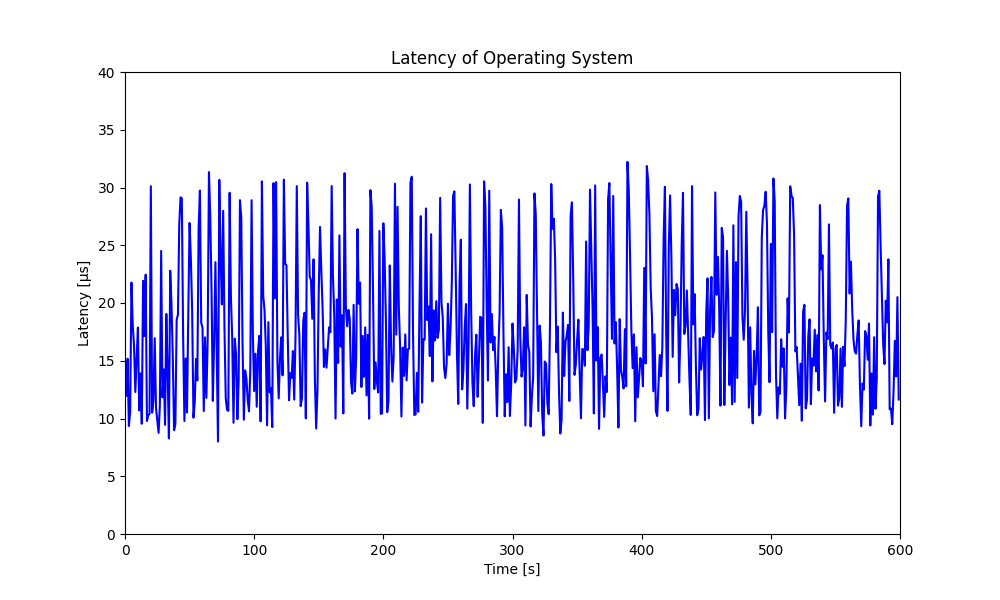
\includegraphics[width=1.0\columnwidth]{masterthesis-documentation/docs/sigmatek/xenomai/3rt/max_latency_rt/max_latency_rt.png}
	\caption[After Article configurations]{After Article configurations}
	\label{fig:max_latency_rt}
\end{figure}

\begin{table}[H]
	\centering
	\caption[Latency statistics of Salamander 4 after BIOS configurations]{Latency statistics of Salamander 4 virtualization after BIOS configurations in microseconds}
	\label{tab:latency_statistics_bios}
	\setlength{\tabcolsep}{0.5em} % for the horizontal padding
	{\renewcommand{\arraystretch}{1.2}% for the vertical padding
		\begin{tabular}{|c|c|}\hline
			\textbf{Statistic} & \textbf{Value (\textmu s)} \\\hline
			Average Latency    & 17.68                      \\\hline
			Maximum Latency    & 32.21                      \\\hline
			Minimum Latency    & 8.005                      \\\hline
			Standard Deviation & 6.1                        \\\hline
		\end{tabular}}
\end{table}



\section{BIOS Configurations}\label{sec:bios_configurations}

BIOS stands for Basic Input/Output System. It abstracts the hardware and enables basic functions of a computer during the booting process, such as starting the operating system and loading other software. Since the BIOS is embedded very deep, its configuration can significantly influence the real-time performance of the system. Table~\ref{tab:bios_configuration} illustrates the specific BIOS settings that have been adjusted for the purpose of real-time performance.

\begin{table}[H]
	\centering
	\caption{BIOS Configurations}
	\label{tab:bios_configuration}
	\setlength{\tabcolsep}{0.5em} % for the horizontal padding
	{\renewcommand{\arraystretch}{1.2}% for the vertical padding
		\begin{tabular}{|l|l|}
			\hline
			\textbf{Option}               & \textbf{Status} \\
			\hline
			Hyper Threading               & Disabled        \\
			\hline
			Intel SpeedStep®              & Disabled        \\
			\hline
			Intel® Speed Shift Technology & Disabled        \\
			\hline
			C States                      & Disabled        \\
			\hline
			VT-d                          & Enabled         \\
			\hline
		\end{tabular}}
\end{table}

\noindent In the following, these settings along with their impact on system latency are briefly described.

\begin{itemize}
	\item \textbf{Hyper Threading}: Hyper-Threading allows CPUs to process two threads simultaneously instead of just one. When it is enabled on the host, this allows the parallelisation of tasks and increases performance. However, in a real-time system like the guest Salamander 4, this can lead to increased latencies due to contention between threads. In order to ensure more deterministic behavior in the guest, it is disabled on the host.
	\item \textbf{Intel SpeedStep}: This technology dynamically adjusts the clock speed of the CPU based on workload. These dynamic changes can lead to unpredictable latencies in a real-time system. It is also disabled on the host to maintain a constant CPU speed.
	\item \textbf{Intel® Speed Shift Technology}: Similar to SpeedStep, Speed Shift allows the processor to directly control its frequency and voltage. This can lead to unpredictable latencies, too. Hence, it is also disabled on the host.
	\item \textbf{C States}: These are low-power idle states where the clock frequency and voltage of the CPU are reduced. Transitioning between C-states can cause variable latencies. To prevent this from happening, C-states are disabled on the host.
	\item \textbf{VT-d}: Direct access to physical devices from within virtual machines is possible when VT-d is enabled on the host. This can help reduce latencies associated with I/O operations in the virtual machine. It is therefore enabled on the host.
\end{itemize}




\section{Kernel Configurations}\label{sec:kernel_configurations}

The kernel command-line parameters are shown in Code~\ref{script:kernel_cli} below.

\vspace{1em}
\begin{minipage}{0.95\columnwidth}
	\begin{lstlisting}[name={Kernel Configuration},label={script:kernel_cli}]
		GRUB_CMDLINE_LINUX="isolcpus=4 rcu_nocbs=4 rcu_nocb_poll nohz_full=4 nohz=on default_hugepagesz=1G hugepagesz=1G hugepages=8 intel_iommu=on rdt=l3cat nmi_watchdog=0 idle=poll clocksource=tsc tsc=reliable audit=0 skew_tick=1 intel_pstate=disable intel.max_cstate=0 intel_idle.max_cstate=0 processor.max_cstate=0 processor_idle.max_cstate=0 nosoftlockup no_timer_check nospectre_v2 spectre_v2_user=off kvm.kvmclock_periodic_sync=N kvm_intel.ple_gap=0 irqaffinity=0"
\end{lstlisting}
\end{minipage}

\noindent In the following, these settings along with their impact on system latency are briefly described.

\begin{itemize}
	\item \textbf{isolcpus=4}: Isolates CPU 4 from the general scheduler, meaning no process will be scheduled to run on this CPU unless it is explicitly assigned. CPU isolation is explained in detail in Section~\ref{subsec:cpu_isolation}.
	\item \textbf{rcu\_nocbs=4}: The Linux kernel uses a synchronization mechanism called RCU, or Read-Copy-Update. It lets writers update the data in a way that guarantees readers will always see the same version while enabling multiple readers to access shared data without locks. The RCU subsystem uses callback functions that need to be invoked once readers are done with the data they accessed. By default, these callbacks are handled by the CPUs that executed the read-side critical sections. This parameter offloads RCU callback handling from CPU 4 to other CPUs. CPU 4 remains dedicated to high-priority tasks which helps in reducing latency.
	\item \textbf{rcu\_nocb\_poll}: This is used together with \texttt{rcu\_nocbs} and causes the system to actively poll for RCU callbacks to invoke, instead of waiting for the next RCU grace period. This reduces latency.
	\item \textbf{nohz\_full=4}: Makes CPU core 4 ``tickless'', meaning the kernel tries to avoid sending periodic scheduling-clock interrupts to the CPU when there are no runnable tasks. This lowers latency by reducing unnecessary wake-ups but may increase power consumption because the CPU is not able to enter a low-power state when idle. Additionally, timer interrupts cannot be fully eliminated because certain events, such as incoming interrupts or task activations, can still cause the kernel to send timer interrupts to the tickless CPU.
	\item \textbf{nohz=on}: Sets all CPUs to tickless mode system-wide.
	\item \textbf{default\_hugepagesz=1G, hugepagesz=1G, hugepages=8}: Huge pages are large contiguous areas of memory that can be used by applications and the kernel, instead of the traditional 4KB small pages. The default huge page size is set to 1GB, and 8 huge pages of 1GB size are reserved at boot. This pre-allocation makes sure that these large memory regions are available to be used by the kernel or applications, without having to dynamically allocate and potentially fail.
	\item \textbf{intel\_iommu=on}: Enables Intel's IOMMU (Input/Output Memory Management Unit), which connects a DMA (Direct Memory Access)-capable I/O bus, such as graphics cards and network adapters, to the main memory. It can enhance device performance by allowing these devices to directly access and use memory, which is especially helpful when these devices are virtualized.
	\item \textbf{rdt=l3cat}: Activates the L3 CAT (L3 Cache Allocation Technology) feature of Intel’s RDT (Resource Director Technology). Unlike L1 and L2 caches, where each core has its fixed capacity, L3 cache is a shared pool among multiple cores. L3 CAT is a mechanism that controls the amount of L3 cache that a process can use. By controlling cache allocation, it can prevent a single process from monopolizing the L3 cache, which is particularly beneficial in virtualized environments, where multiple virtual machines share the same physical host.
	\item \textbf{nmi\_watchdog=0}: Disables the NMI (Non-Maskable Interrupt) watchdog, which is a debugging feature of the Linux kernel. It works by periodically generating non-maskable interrupts. If the system does not respond to these interrupts within a certain timeframe, the NMI watchdog concludes that the system has hung and generates a system dump for debugging.  This constant monitoring consumes CPU cycles and can introduce undesirable latency in real-time systems.
	\item \textbf{idle=poll}: Changes the CPU’s idle loop behavior to active polling. Instead of entering a low-power state when idle, the CPU continuously polls for new tasks. This can reduce task start latency in real-time systems, but it increases power consumption.
	\item \textbf{clocksource=tsc, tsc=reliable}: TSC (Time Stamp Counter) is a high-resolution timer provided by most x86 processors that counts the number of CPU cycles since it was last reset. Accurate timekeeping is crucial, particularly for real-time systems. These parameters set the clocksource to TSC and mark it as a reliable source of timekeeping, meaning it increments at a consistent rate and does not stop when the processor is idle.
	\item \textbf{audit=0}: Disables the Linux audit system. When it is enabled, it generates log entries for security-relevant events, which is a slow operation since they are written to disk. If there are a large number of such events, the audit system can consume significant CPU time and I/O bandwidth which could lead to higher latency.
	\item \textbf{skew\_tick=1}: Enables a mode in the Linux kernel that reduces timer interrupt overhead. Normally, timer interrupts happen simultaneously on all CPUs, resulting in all CPUs to exit their low-power states at once. This can lead to increased contention for system resources. When enabled, the kernel offsets the timer interrupts on different CPUs, spreading them out over time.
	\item \textbf{intel\_pstate=disable}: Disables the Intel P-state driver, which is a part of the Linux kernel that handles power management for Intel CPUs. It controls the frequency of the CPU by scaling it up when demand is high and scaling it down to save power when demand is low. This dynamic frequency scaling is disabled because it leads to increased latencies for real-time systems.
	\item \textbf{intel.max\_cstate=0, intel\_idle.max\_cstate=0, processor.max\_cstate=0, processor\_idle.max\_cstate=0}: These parameters disable deeper C-states (CPU power saving states). Normally, when a CPU is idle, it can enter various C-states, with higher-numbered states representing deeper sleep states that save more power but take longer to wake up from. In real-time systems, these wake-up delays can be problematic. Disabling them leads keeps the CPUs ready to respond quickly to new tasks and helps in reducing latency.
	\item \textbf{nosoftlockup}: Disables the soft lockup detector in the Linux kernel. A soft lockup is when a CPU is busy executing kernel code for a long period of time without giving other tasks a chance to run. Especially threads with SCHED\_FIFO policy occupy the CPU for an extensive duration. This is detected and reported by the soft lockup detector, hence it is disabled to prevent these unnecessary warnings.
	\item \textbf{no\_timer\_check}: Disables the check for broken timer interrupt sources. Broken timer interrupt sources are problems with hardware or software that prevent timer interrupts from working as intended. Such a timer may not generate interrupts at the expected rate or at all. The kernel skips the checks for these broken timer interrupt sources, which can cause unnecessary overhead in a real-time system where every CPU cycle counts.
	\item \textbf{nospectre\_v2, spectre\_v2\_user=off}: These parameters disable mitigations for the Spectre v2 vulnerability. Spectre v2 is a hardware vulnerability that affects many modern microprocessors and can allow malicious programs to access sensitive data they are not supposed to. While this is necessary for security, it has an impact on performance and should be turned off in controlled environments where the risk of exploitation is low.
	\item \textbf{kvm.kvmclock\_periodic\_sync=N, kvm\_intel.ple\_gap=0}: These are KVM (Kernel-based Virtual Machine) related parameters. They disable the periodic synchronization of the kvmclock and set the gap between PLE (Pause Loop Exiting) events to 0. The kvmclock is a paravirtualized clock source provided by KVM to its guest OS and disabling this reduces latency introduced by clock synchronization. By setting the gap to 0, the virtual machine exits the pause loop immediately, which can reduce latency in spinlock-intensive workloads.
	\item \textbf{irqaffinity=0}: Sets the default Interrupt Request affinity to none. This means that no CPU core is preferred over another for handling IRQs. Instead, it lets the operating system decide how to distribute these IRQs across all the CPUs. Section~\ref{subsec:irq_handling} dives deeper into Interrupt Request affinity.
\end{itemize}

\textcolor{red}{After the BIOS and Kernel configurations, Figure~\ref{fig:max_latency_rt_kernelparam}}

\begin{figure}[H]
	\centering
	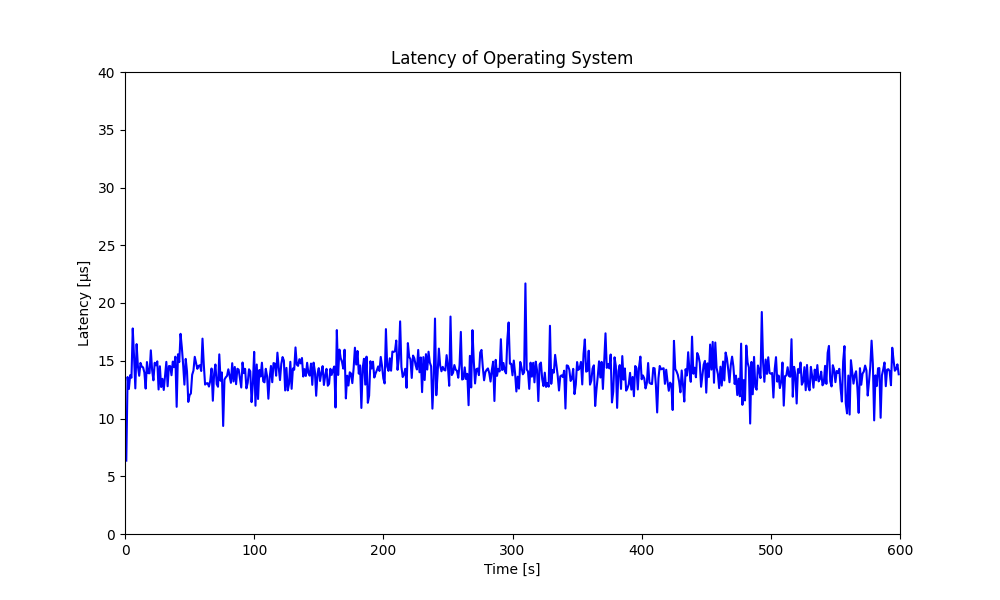
\includegraphics[width=1.0\columnwidth]{masterthesis-documentation/docs/sigmatek/xenomai/4rt_kernelparam/max_latency_rt_kernelparam/max_latency_rt_kernelparam.png}
	\caption[After BIOS and Kernel configurations]{After BIOS and Kernel configurations}
	\label{fig:max_latency_rt_kernelparam}
\end{figure}

\begin{table}[H]
	\centering
	\caption[Latency statistics of Salamander 4 after Kernel configurations]{Latency statistics of Salamander 4 virtualization after Kernel configurations in microseconds}
	\label{tab:latency_statistics_kernel}
	\setlength{\tabcolsep}{0.5em} % for the horizontal padding
	{\renewcommand{\arraystretch}{1.2}% for the vertical padding
		\begin{tabular}{|c|c|}\hline
			\textbf{Statistic} & \textbf{Value (\textmu s)} \\\hline
			Average Latency    & 14.00                      \\\hline
			Maximum Latency    & 21.694                     \\\hline
			Minimum Latency    & 6.351                      \\\hline
			Standard Deviation & 1.44                       \\\hline
		\end{tabular}}
\end{table}



\section{Host OS Configurations}\label{sec:host_configurations}
The host OS needs to provide an environment where the guest OS can operate in real-time. This entails a number of host-side adjustments to reduce interruptions and reduce latency. In the following, a detailed overview of these configurations and their impact on the real-time performance of the guest OS is provided.
\subsection{CPU affinity and Isolation}\label{subsec:cpu_isolation}

Isolating CPUs involves removing all user-space threads and unbound kernel threads since bound kernel threads are tied to specific CPUs and hence cannot be moved. For CPU isolation, the~\texttt{isolcpus} function was used to isolate a performance CPU from the general scheduling algorithms of the operating system. This means that the isolated CPUs will not be used for regular task scheduling, allowing them to be dedicated for the real-time specific tasks. However, the isolcpus function only isolates at the user level and does not affect kernel tasks. Consequently, these kernel tasks and interrupts can still utilize the CPU~\cite{maPerformanceTuningKVMbased}, including systemd services. To prevent systemd services from running on an isolated CPU, the CPU affinity can be set the with line \texttt{CPUAffinity=0 1 2 3 5 6 7 8 9 10 11 12 13} in the \texttt{/etc/systemd/system.conf} file to indicate the CPUs that systemd-services are allowed to run on. Every CPU other than the isolated CPU 4 is allowed. Code~\ref{output:pse} shows the user and kernel tasks that run on CPU 4. After the isolation, user tasks other than the QEMU process have been removed from running on this CPU. Only few per-CPU kernel threads that are tied to this CPU still take CPU time.

\vspace{1em}
\begin{minipage}{0.95\columnwidth}
	\begin{lstlisting}[name={User and Kernel Tasks},label={output:pse},escapeinside={(*@}{@*)}]
		sigma_ibo@sigma-ibo:~$ cat /sys/devices/system/cpu/isolated
		4
		sigma_ibo@sigma-ibo:~$ ps axHo psr,pid,lwp,args,policy,nice,rtprio | awk '$1 == 4'
		4      38      38 [cpuhp/4]                   TS    0      -
		4      39      39 [idle_inject/4]             FF    -     50
		4      40      40 [migration/4]               FF    -     99
		4      41      41 [ksoftirqd/4]               TS    0      -
		4      42      42 [kworker/4:0-events]        TS    0      -
		4      43      43 [kworker/4:0H-kblockd]      TS  -20      -
		4     153     153 [kworker/4:1-events]        TS    0      -
		4   81649   81649 qemu-system-x86_64 -M pc,ac TS    0      -
		4   81649   81654 qemu-system-x86_64 -M pc,ac TS    0      -
		4   81649   81676 qemu-system-x86_64 -M pc,ac TS    0      -
		4   81649   81702 qemu-system-x86_64 -M pc,ac TS    0      -
		4   81649   82185 qemu-system-x86_64 -M pc,ac TS    0      -
		4   81649   82187 qemu-system-x86_64 -M pc,ac TS    0      -
		4   82134   82134 [kworker/4:1H-kblockd]      TS  -20      -
\end{lstlisting}
\end{minipage}
\subsection{KVM Entry and KVM Exit}\label{subsec:kvm_entry_exit}
\textcolor{red}{\noindent Upon isolating a CPU to the QEMU process, it was anticipated that the guest would utilize nearly 100\% of the CPU's capacity, with minimal to no intervention from the host. However, the isolcpus function only isolates CPUs from the scheduler, meaning that user-space processes won't be scheduled on these CPUs, but kernel tasks and interrupts can still utilize the CPU.This led to the investigation of the causes for the observed high and inconsistent latency. The guest operates within the~\texttt{kvm\_entry} and~\texttt{kvm\_exit} events of the host. Kernelshark revealed a high frequency of~\texttt{kvm\_exit} events, indicating that the guest frequently relinquishes control of the CPU back to the host. This frequent switching hinders the guest's ability to run continuously, thereby increasing the virtualization latency.}

\textcolor{red}{To further understand this, trace-cmd was employed to trace various events in the host-guest communication, including the reasons for these events. Specifically, the causes for~\texttt{kvm\_exit} events were analyzed. The command sudo trace-cmd record -e all -A @3:823 --name Salamander4 -e all was executed on the host for a duration of 5 seconds. The results in Figure~\ref{fig:kvm_exit_taskset} were obtained. Additionally, Table~\ref{tab:kvm_exit} provides a short description of the observed~\texttt{kvm\_exit} events.}

\begin{table}[H]
	\centering
	\begin{tabular}{|l|p{0.62\textwidth}|}
		\hline
		\textbf{Exit Reason} & \textbf{Description}                                     \\ \hline
		APIC\_WRITE          & Triggered when the guest writes to its APIC.             \\ \hline
		EXTERNAL\_INTERRUPT  & Triggered by external hardware interrupts.               \\ \hline
		HLT                  & Triggered when the guest executes the HLT instruction.   \\ \hline
		EPT\_MISCONFIG       & Triggered by a misconfiguration in the EPT.              \\ \hline
		PREEMPTION\_TIMER    & Triggered when the host's preemption timer expires.      \\ \hline
		PAUSE\_INSTRUCTION   & Triggered when the PAUSE instruction is executed.        \\ \hline
		EPT\_VIOLATION       & Triggered by a violation of the EPT permission settings. \\ \hline
		IO\_INSTRUCTION      & Triggered when the guest executes an I/O instruction.    \\ \hline
		EOI\_INDUCED         & Triggered when an EOI signal is sent to the APIC.        \\ \hline
		MSR\_READ            & Triggered when the guest reads from a MSR.               \\ \hline
		CPUID                & Triggered when the guest executes the CPUID instruction. \\ \hline
	\end{tabular}
	\caption{Description of kvm\_exit reasons}
	\label{tab:kvm_exit}
\end{table}

\textcolor{red}{\noindent In the process of analyzing the~\texttt{kvm\_exit} events, several reasons for these exits were identified. The most frequent among these were the~\texttt{APIC\_WRITE} and~\texttt{HLT} events. The former is initiated when the guest writes to its Advanced Programmable Interrupt Controller (APIC), a component of the CPU that manages hardware interrupts. The latter occurs when the guest executes the HLT instruction, effectively halting the CPU until the next external interrupt is fired. Other significant but less frequent events included~\texttt{EXTERNAL\_INTERRUPT} and~\texttt{IO\_INSTRUCTION}. These events are indicative of the guest's interaction with hardware devices and its execution of I/O operations. Events such as~\texttt{EPT\_MISCONFIG} and~\texttt{PREEMPTION\_TIMER} were also noted. These could potentially signal issues with memory management and the host's scheduling of the guest. While events like~\texttt{PAUSE\_INSTRUCTION},~\texttt{EPT\_VIOLATION},~\texttt{EOI\_INDUCED},~\texttt{MSR\_READ}, and~\texttt{CPUID} were the least frequent, they still provide valuable insights into the guest's behavior and the host-guest interaction.}

\textcolor{red}{\noindent When the script is started from the host, the QEMU process can be scheduled to run on any available core, as it is not bound to a specific CPU core. This means that the QEMU process may frequently switch between different cores, leading to an increase in latency. As the goal was to reduce latency in the guest, the first step was to isolate a CPU of the host and dedicate it solely to the QEMU process, so that it cannot be used for other tasks on the user level. Without CPU isolation, context switches take place at the operating system level and not at the hypervisor level. This explains why there are fewer~\texttt{kvm\_exit} events. However, this will also, as previously shown, lead to higher latency, as context switches at the operating system level generally take longer than a~\texttt{kvm\_exit} and ~\texttt{kvm\_entry}. When the CPU was dedicated to the QEMU process, on the other hand, there was a significant increase in~\texttt{kvm\_exit} events. This is because every context switch takes place at the hypervisor level. Nevertheless, lower latency was achieved thereby, as the qemu process is no longer influenced by the CPU scheduling of the operating system.}

\subsection{Interrupt Affinity}\label{subsec:irq_handling}
Once the CPUs were isolated, interrupt requests handling was the next step. The purpose of interrupt requests is to inform the CPU to stop working on a certain job and start working on another. This allows hardware devices to communicate with the CPU through frequent context switches, which can introduce latency in real-time systems. The~\texttt{/proc/interrupts} file can be monitored using the command~\texttt{watch -d -n 1 cat /proc/interrupts} to observe changes in the interrupt requests handled by each CPU in real-time. The IRQs needed to be removed from the isolated CPU by manipulating the~\texttt{/proc/irq/<IRQ>/smp\_affinity} files. The value in the~\texttt{smp\_affinity} file is a bitmask in hexadecimal format where each bit corresponds to a CPU. The least significant bit (LSB) on the right corresponds to the first CPU (CPU0), and the most significant bit (MSB) on the left corresponds to the last CPU (CPU13). When there are 14 CPUs available, the default value for~\texttt{smp\_affinity} would be 3FFF. Removing CPU 4 out of this bitmask would be setting bit five to zero, resulting in 3FEF (11 1111 1110 1111). The python script in Code~\ref{script:smp_affinity} was written to show a table of the distribution of interrupt requests across each CPU. By changing the values of the~\texttt{smp\_affinity} files, the assignment of IRQs to CPUs is controlled.


\vspace{1em}
\begin{minipage}{0.95\columnwidth}
	\begin{lstlisting}[name={Check distribution of interrupt requests across each CPU},label={script:smp_affinity}]
		import os
		import pandas as pd
		from tabulate import tabulate
		
		# Get the number of CPUs
		num_cpus = os.cpu_count()
		
		# Initialize a dictionary to store the CPUs for each IRQ
		irqs = {}
		
		# Iterate over each IRQ
		for irq in os.listdir('/proc/irq'):
			# Check if the smp_affinity file exists for this IRQ
			if os.path.isfile(f'/proc/irq/{irq}/smp_affinity'):
				# Read the current smp_affinity
				with open(f'/proc/irq/{irq}/smp_affinity', 'r') as f:
					affinity = int(f.read().strip(), 16)
				# Initialize an empty list to store the CPUs for this IRQ
				cpus = []
				# Iterate over each CPU
				for cpu in range(num_cpus):
					# Check if the bit for the current CPU is set
					if ((affinity & (1 << cpu)) != 0):
						# Add the CPU to the list for this IRQ
						cpus.append(cpu)
				# Sort the list of CPUs
				cpus.sort()
				# Add the list of CPUs to the dictionary for this IRQ
				irqs[irq] = cpus
		
		# Create a DataFrame to store the table
		df = pd.DataFrame(index=sorted(irqs.keys(), key=int), columns=range(num_cpus))
		
		# Fill the DataFrame with 'x' where a CPU is assigned to an IRQ
		for irq, cpus in irqs.items():
			for cpu in cpus:
				df.loc[irq, cpu] = 'x'
		
		# Replace NaN values with empty strings
		df.fillna('', inplace=True)
		
		# Print the table in pipe format
		print(tabulate(df, headers='keys', tablefmt='pipe', showindex=True))
		
		# Convert the DataFrame to a markdown table
		markdown_table = df.to_markdown()
		
		# Write the markdown table to a file
		with open('table_CPU_IRQ.md', 'w') as f:
			f.write(markdown_table)
\end{lstlisting}
\end{minipage}


\noindent However, as the proc filesystem resets to its default state after each reboot, manually changing numerous IRQ files is tedious and time-consuming. This process was automated using the shell script in Code~\ref{script:change_smp_affinity}, which is executed after every reboot. Additionally, the CPU affinity of IRQ threads of NVME (Non-Volatile Memory Express, a type of SSD storage) can be set away from CPU 4 to avoid impacting real-time workloads. This can be done through finding out the respective process IDs through \texttt{ps -e | grep irq/.*nvme} and then executing \texttt{sudo taskset -a -p -c 0 <PID>}.

\vspace{1em}
\begin{minipage}{0.95\columnwidth}
	\begin{lstlisting}[name={Change IRQ assignment of a CPU},label={script:change_smp_affinity}]
		#!/bin/bash

		# Check if a command-line argument is provided
		if [ -z "$1" ]; then
			echo "Please provide a CPU number as a command-line argument."
			exit 1
		fi
		
		# Get the CPU number from the command-line argument
		CPU=$1
		
		# Define the mask values
		declare -A mask_values
		mask_values=( [0]="3ffe" [1]="3ffd" [2]="3ffb" [3]="3ff7" [4]="3fef" [5]="3fdf" [6]="3fbf" [7]="3f7f" [8]="3eff" [9]="3dff" [10]="3bff" [11]="37ff" [12]="2fff" [13]="17ff")
		
		# Run the check_smp_affinity.sh script and get the IRQs
		IRQs=$(./check_smp_affinity.sh $CPU | grep -o '[0-9]\+')
		
		# Initialize an empty array to store the IRQs that could not be removed
		failed_IRQs=()
		# Initialize an empty array to store the IRQs that were successfully removed
		succeeded_IRQs=()
		
		# Loop over the IRQs
		for IRQ in $IRQs; do
			# Try to change the smp_affinity
			echo ${mask_values[$CPU]} | sudo tee /proc/irq/$IRQ/smp_affinity > /dev/null 2>&1
			# If the command failed, add the IRQ to the failed_IRQs array
			if [ $? -ne 0 ]; then
				failed_IRQs+=($IRQ)
			else
				succeeded_IRQs+=($IRQ)
			fi
		done
		
		# Check if there were any failed IRQs
		if [ ${#failed_IRQs[@]} -ne 0 ]; then
			echo "IRQs ${failed_IRQs[@]} could not be removed from CPU $CPU."
		fi
		
		# Check if there were any successful IRQs
		if [ ${#succeeded_IRQs[@]} -ne 0 ]; then
			# Remove the first entry from the succeeded_IRQs array
			succeeded_IRQs=("${succeeded_IRQs[@]:1}")
			echo "IRQs ${succeeded_IRQs[@]} were removed from CPU $CPU."
		fi		
\end{lstlisting}
\end{minipage}
\subsection{RT-Priority}
Having a real-time kernel itself is a crucial part of achieving deterministic behavior, but not enough to take full advantage of the real-time capabilities. One key aspect of this are real-time priorities, thoroughly explained by Richard Weinberger in~\cite{LinuxProcessPriorities}. In essence, Table~\ref{tab:scheduling_priorities} lists minimum and maximum priorities for different scheduling policies in Linux.

\begin{table}[H]
	\centering
	\caption{Minimum and maximum priorities for different scheduling policies}
	\label{tab:scheduling_priorities}
	\setlength{\tabcolsep}{0.5em} % for the horizontal padding
	{\renewcommand{\arraystretch}{1.2}% for the vertical padding
		\begin{tabular}{|l|l|l|}
			\hline
			\textbf{Scheduling Policy} & \textbf{Min Priority} & \textbf{Max Priority} \\ \hline
			SCHED\_OTHER               & 0                     & 0                     \\ \hline
			SCHED\_FIFO                & 1                     & 99                    \\ \hline
			SCHED\_RR                  & 1                     & 99                    \\ \hline
			SCHED\_BATCH               & 0                     & 0                     \\ \hline
			SCHED\_IDLE                & 0                     & 0                     \\ \hline
			SCHED\_DEADLINE            & 0                     & 0                     \\ \hline
		\end{tabular}}
\end{table}

\noindent \texttt{SCHED\_FIFO} allows deterministic, high-priority execution of critical tasks without being preempted by lower-priority processes. The virtual machine can either be started with \texttt{chrt -f <PRIO>} or adjusted at a later point with \texttt{chrt -f <PRIO> <PID>}. It is also important that there are no other unexpected real time processes running on the system concurrently.
\subsection{Disable RT Throttling}
If a real-time task consumes 100\% of the CPU time, the system may become unresponsive as a whole. This happens because an RT process is constantly using the CPU and the Linux scheduler will not schedule other non-RT processes in the meantime. To prevent complete system lockups, the kernel has a function to throttle RT processes if they consume 0.95 seconds out of every 1 second of CPU time. It does this by pausing the process for the remaining 0.05 seconds, which is not desired because this could result in missed deadlines. RT throttling can be disabled by  writing the value -1 to the~\texttt{/proc/sys/kernel/sched\_rt\_runtime\_us} file. This change also needs to be made permanent because the proc filesystem resets to its default state after each reboot. For this purpose, the line~\texttt{kernel.sched\_rt\_runtime\_us = -1} can be appended to the end of the~\texttt{/etc/sysctl.conf} file, which is read at boot time and used to configure kernel parameters. This reduces the potential for missed deadlines.
\subsection{Disable Timer Migration}
Timer migration allows timers to be moved from one CPU to another, which means the kernel can balance load across multiple CPUs. In a real-time system, this can introduce latency and jitter. To disable timer migration, the value ``0'' needs to be written to the~\texttt{/proc/sys/kernel/timer\_migration} file. This change also needs to be made permanent by writing the line~\texttt{kernel.timer\_migration = 0} to the~\texttt{/etc/sysctl.conf} file. This reduces the amount of context switches and interrupts.
\subsection{Set Device Driver Work Queue}
The device driver work queue allows time-consuming tasks to be offloaded to be processed later in a separate kernel thread. By setting the work queue away from CPU 4 to another CPU, it is free to handle real-time tasks without being interrupted by these work queue tasks. This is done by specifying a bitmask to exclude CPU 4 in the files \texttt{/sys/devices/virtual/workqueue/cpumask} and \texttt{/sys/bus/workqueue/devices/writeback/cpumask}.
\subsection{Disable RCU CPU Stall Warnings}
As already mentioned in Section~\ref{sec:kernel_configurations}, the Linux kernel uses RCU as a synchronization mechanism for reading from and writing to shared data. An RCU CPU stall in the Linux kernel can occur due to several reasons. These include a CPU looping in an RCU read-side critical section, a CPU looping with interrupts disabled, a CPU looping with preemption disabled, or a CPU not getting around to less urgent tasks, known as “bottom halves”. The number of seconds the kernel should wait before checking for stalled CPUs and reporting a stall warning can be set via the ~\texttt{/sys/module/rcupdate/parameters/rcu\_cpu\_stall\_timeout} file. These warnings can be suppressed alltogether to reduce the potential for increased latency by writing ``1'' to the~\texttt{/sys/module/rcupdate/parameters/rcu\_cpu\_stall\_suppress} file. This setting is also not persistent across reboots, so the command needs to be added to a startup script.
\subsection{Stop Certain Services}
Services like irqbalance.service, thermald.service, and wpa\_supplicant.service, as presented in Table~\ref{tab:stop_servies} can be further sources for random latency and unnecessary overhead. Stopping these services through \texttt{sudo systemctl stop <SERVICE>} means they will not be able to interrupt the CPU with their tasks.

\begin{table}[H]
	\centering
	\caption{Description of Services}
	\label{tab:stop_servies}
	\setlength{\tabcolsep}{0.5em} % for the horizontal padding
	{\renewcommand{\arraystretch}{1.2}% for the vertical padding
		\begin{tabular}{|l|l|}
			\hline
			\textbf{Service}        & \textbf{Description}                        \\
			\hline
			irqbalance.service      & Distributes hardware interrupts across CPUs \\\hline
			thermald.service        & A daemon that prevents overheating          \\\hline
			wpa\_supplicant.service & A service for wireless network devices      \\
			\hline
		\end{tabular}}
\end{table}
\subsection{Disable Machine Check}
Machine checks report hardware errors and these checks can cause interruptions and increase latency. Hence it is best to disable them in real-time scenarios by writing a ``0'' to the \texttt{/sys/devices/system/machinecheck/machinecheck0/check\_interval} file.

\subsection{Boot into text-based environment}
The Graphical User Interface (GUI) consumes great amounts of system resources. It often runs different background processes that are not essential for real-time systems and hence increase latency. These resources can be freed up by switching to a text-based environment. This way, processing power and memory can be allocated to critical real-time tasks which in turn can lead to lower latency and deterministic behavior. The command \texttt{systemctl set-default multi-user.target} and a following reboot allow for booting into a text-based environment. For the sake of completeness, the graphical interface can be brought back through the command \texttt{systemctl set-default graphical.target} and a following reboot.

\textcolor{red}{After the Host configurations, Figure~\ref{fig:max_latency_rt_kernelparam_host}}

\begin{figure}[H]
	\centering
	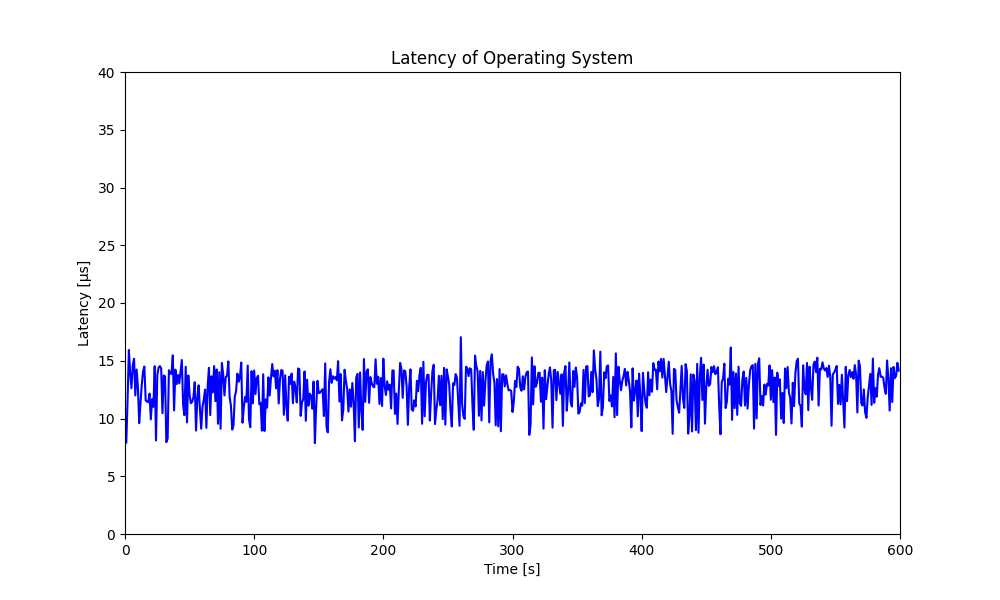
\includegraphics[width=1.0\columnwidth]{masterthesis-documentation/docs/sigmatek/xenomai/5rt_kernelparam_host/max_latency_rt_kernelparam_host/max_latency_rt_kernelparam_host.png}
	\caption[After Host configurations]{After Host configurations}
	\label{fig:max_latency_rt_kernelparam_host}
\end{figure}

\begin{table}[H]
	\centering
	\caption[Latency statistics of Salamander 4 after Host configurations]{Latency statistics of Salamander 4 virtualization after Host configurations in microseconds}
	\label{tab:latency_statistics_host}
	\setlength{\tabcolsep}{0.5em} % for the horizontal padding
	{\renewcommand{\arraystretch}{1.2}% for the vertical padding
		\begin{tabular}{|c|c|}\hline
			\textbf{Statistic} & \textbf{Value (\textmu s)} \\\hline
			Average Latency    & 12.61                      \\\hline
			Maximum Latency    & 17.041                     \\\hline
			Minimum Latency    & 7.872                      \\\hline
			Standard Deviation & 1.8                        \\\hline
		\end{tabular}}
\end{table}


\section{QEMU/KVM Configurations}\label{sec:guest_configurations}
KVM allows the guest OS to run directly on the hardware, bypassing the need for traditional emulation which can introduce delays. QEMU, when used with KVM, provides hardware-assisted virtualization, which also lowers latency in the guest OS.

\subsection{Tune LAPIC Timer Advance}
The Local Advanced Programmable Interrupt Controller (LAPIC) is a built-in timer that handles the delivery of interrupts to the CPU.
It generates interrupts at a rate. This rate can be tuned in the \texttt{/sys/module/kvm/parameters/lapic\_timer\_advance\_ns} file to reduce the frequency of interrupts and therefore decrease the latency of the guest VM. The default value is ``-1'', which means that the kernel will automatically calculate an appropriate advance for the timer. Here, it is set to the value ``7500''. Hence,the timer interrupt will be delivered 7500 nanoseconds earlier than it is actually due. This gives the VM more time to handle it.

\subsection{Set QEMU Options for real-time VM}
QEMU provides several options that can be used to improve the real-time performance of the guest VM. Table~\ref{tab:qemu_options} briefly explains these options.

\begin{table}[H]
	\centering
	\caption{QEMU options for real-time performance}
	\label{tab:qemu_options}
	\setlength{\tabcolsep}{0.5em} % for the horizontal padding
	{\renewcommand{\arraystretch}{1.2}% for the vertical padding
		\begin{tabular}{|p{6.5cm}|p{8cm}|}
			\hline
			\textbf{QEMU Option}                                                             & \textbf{Description}                                                             \\\hline
			\texttt{-object memory-backend-ram,}\newline\texttt{id=ram0,size=4G,prealloc=on} & Locks the memory of the VM to 4GB and prevents it from being swapped out to disk \\\hline
			\texttt{-mem-prealloc} \newline \texttt{-mem-path /dev/hugepages/}               & Enables the use of hugepages and improves \newline memory access                 \\\hline
		\end{tabular}}
\end{table}

\noindent Code~\ref{script:qemu_def_tuned} shows the final QEMU script used to start the Salamander 4 virtualization, including these options.

\vspace{1em}
\begin{minipage}{\linewidth}
	\begin{lstlisting}[name={Tuned QEMU script for starting Salamander 4 virtualization},label={script:qemu_def_tuned}]
		#!/bin/sh

		if  [ ! -d drive-c/ ]; then
				echo "Filling drive-c/"
				mkdir drive-c/
				tar -C drive-c/ -xf stek-drive-c-image-sigmatek-core2.tar.gz
		fi
			
		exec taskset -c 4 qemu-system-x86_64 -M pc,accel=kvm -kernel ./bzImage \
		-m 2048 -drive file=salamander-image-sigmatek-core2.ext4,format=raw,media=disk \
		-append "console=ttyS0 console=tty1 root=/dev/sda rw panic=1 sigmatek_lrt.QEMU=1 ip=dhcp rootfstype=ext4 schedstats=enable nohlt idle=poll quiet xeno_hal.smi=1 xenomai.smi=1 threadirqs" \
		-net nic,model=e1000,netdev=e1000 -netdev bridge,id=e1000,br=nm-bridge \
		-fsdev local,security_model=none,id=fsdev0,path=drive-c -device virtio-9p-pci,id=fs0,fsdev=fsdev0,mount_tag=/mnt/drive-C \
		-device vhost-vsock-pci,guest-cid=3,id=vsock0 \
		-drive if=pflash,format=qcow2,file=ovmf.code.qcow2 \
		-object memory-backend-ram,id=ram0,size=4G,prealloc=on \
		-mem-prealloc -mem-path /dev/hugepages \
		-no-reboot -nographic
	\end{lstlisting}
\end{minipage}


\textcolor{red}{After the QEMU configurations, Figure~\ref{fig:max_latency_rt_kernelparam_host_qemu}}

\begin{figure}[H]
	\centering
	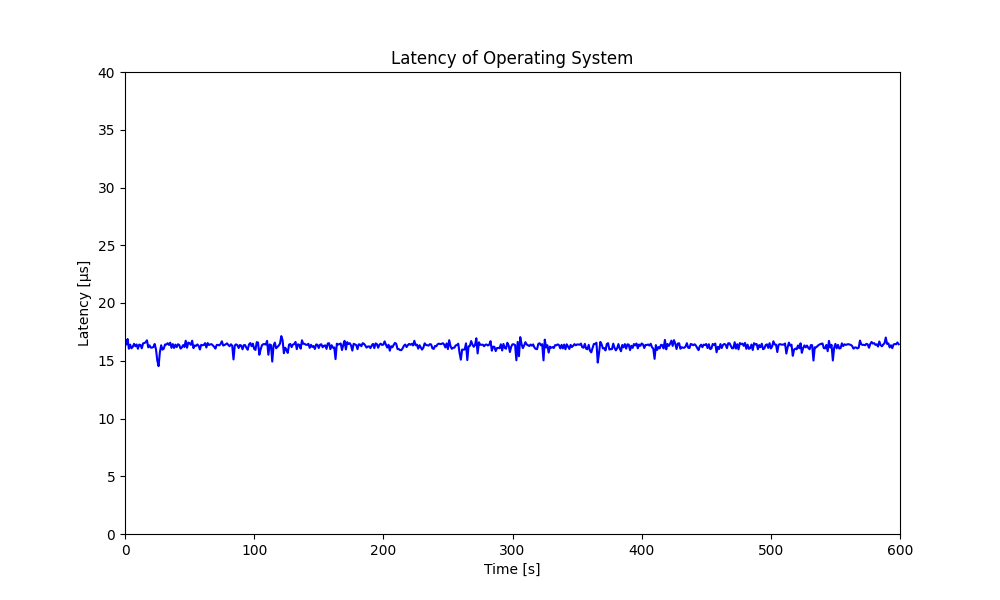
\includegraphics[width=1.0\columnwidth]{masterthesis-documentation/docs/sigmatek/xenomai/6rt_kernelparam_host_qemu/max_latency_rt_kernelparam_host_qemu/max_latency_rt_kernelparam_host_qemu.png}
	\caption[After QEMU configurations]{After QEMU configurations}
	\label{fig:max_latency_rt_kernelparam_host_qemu}
\end{figure}

\begin{table}[H]
	\centering
	\caption[Latency statistics of Salamander 4 after QEMU configurations]{Latency statistics of Salamander 4 virtualization after QEMU configurations in microseconds}
	\label{tab:latency_statistics_qemu}
	\setlength{\tabcolsep}{0.5em} % for the horizontal padding
	{\renewcommand{\arraystretch}{1.2}% for the vertical padding
		\begin{tabular}{|c|c|}\hline
			\textbf{Statistic} & \textbf{Value (\textmu s)} \\\hline
			Average Latency    & 16.26                      \\\hline
			Maximum Latency    & 17.134                     \\\hline
			Minimum Latency    & 14.532                     \\\hline
			Standard Deviation & 0.3                        \\\hline
		\end{tabular}}
\end{table}


\section{Guest OS Configurations}


\section{Other Configurations}
There are other configurations that may be relevant depending on the case. Linux Kernel Developer Steven Rostedt explains all relevant aspects of a real-time system that must be considered in~\cite{kernelrecipesKernelRecipes20162016} and gives insight for finding sources of latency on the linux system in~\cite{thelinuxfoundationFindingSourcesLatency2020}. A Checklist for Writing Linux Real-Time Applications is provided by John Ogness in~\cite{thelinuxfoundationChecklistWritingLinux2020}. Every layer of the system stack must be deterministic to ensure predictable and reliable latency, including hardware, operating system, middleware and drivers, and the application software. ~\cite{HOWTOBuildRTapplication} and~\cite{RealtimeProgrammingLinux} describe the process of writing hard real time Linux programs using the real time preemption patch in great detail. Various hardware and software tunings are mentioned in~\cite{KVMQemuVirtualization} and~\cite{RealTimePerformanceTuning2022}.

\clearpage

\chapter{Real-Time Robotic Application}\label{cha:robotic_application}
This chapter compares the latency of the Salamander 4 operating system before and after the real-time performance tunings with the latency of Salamander 4 running on bare metal hardware. This comparison is done with the aid of a program that will be explained shortly. The goal is to understand how closely the performance of the virtualization can match that of the bare metal. The experimental setup includes a six-axis mini-robot, illustrated in Figure~\ref{fig:mini_robot}.

\begin{figure}[H]
	\centering
	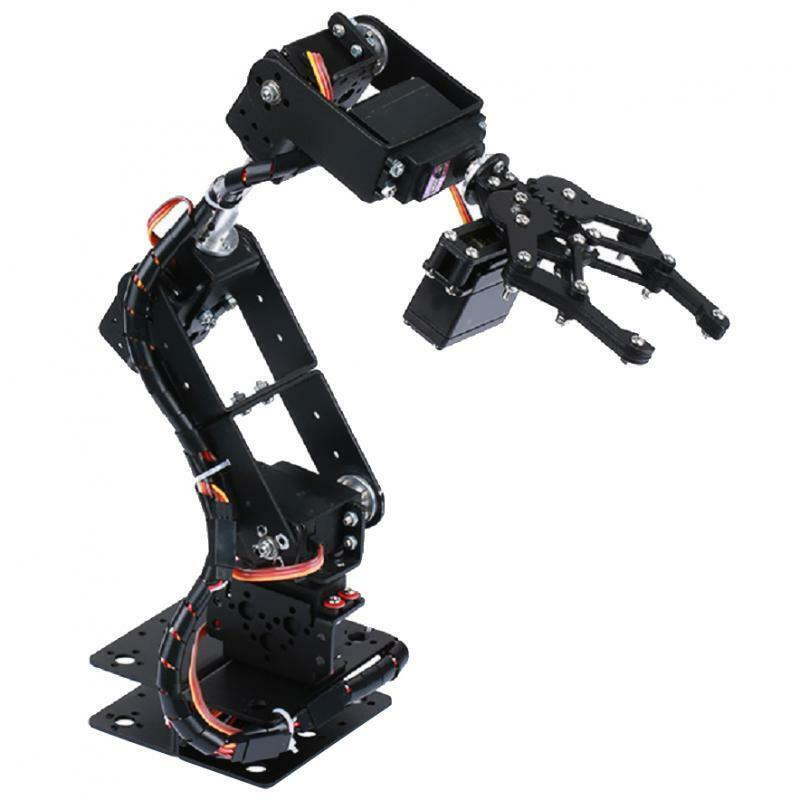
\includegraphics[width=0.45\columnwidth]{img/experiment/mini_robot.jpg}
	\caption[Mini-robot of the experiment]{Mini-robot of the experiment}
	\label{fig:mini_robot}
\end{figure}

\noindent The drive system of the robot arm consists of six MG996R digital servo motors~\cite{MG996RServoMotor}, equipped with a metal gearbox. The motor is able to rotate in a range of approximately 180 degrees and its position can be controlled with a high degree of accuracy. Each servo motor has three wires that need to be connected as shown in Figure~\ref{fig:motor_wires}.

\begin{figure}[H]
	\centering
	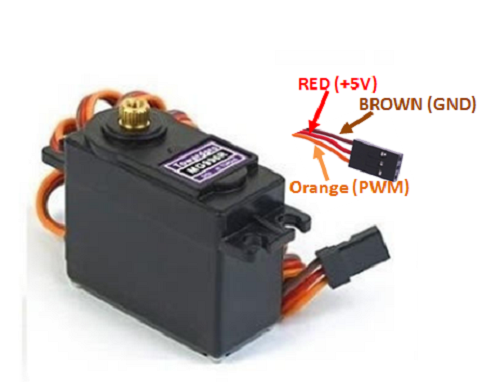
\includegraphics[width=0.45\columnwidth]{img/experiment/motor_wires.png}
	\caption[MG996R Servo Motor]{MG996R Servo Motor~\cite{MG996RServoMotor}}
	\label{fig:motor_wires}
\end{figure}

\noindent To drive the motor, it has to be powered using the red and brown wires and can be controlled by sending PWM signals to the orange wire. In this experiment, this PWM signal is generated by the proprietary PW 022 pulse width module of Sigmatek~\cite{DigitalOutputSIGMATEK}. Its connector layout is illustrated in Figure~\ref{fig:pw022_connectors}.

\begin{figure}[H]
	\centering
	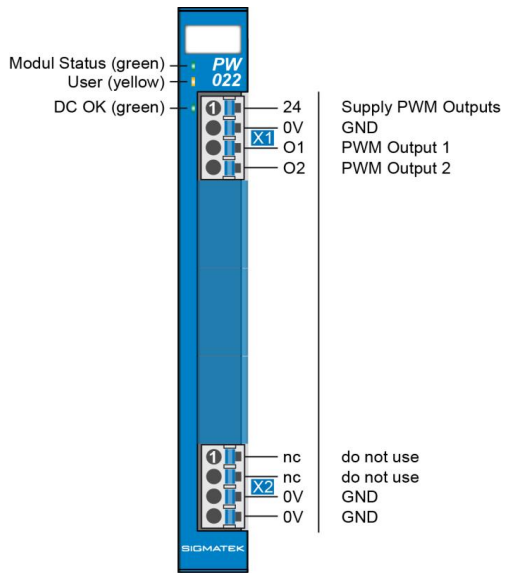
\includegraphics[width=0.5\columnwidth]{img/experiment/pw022_connectors.png}
	\caption[PW 022 pulse width module connector layout]{PW 022 pulse width module connector layout~\cite{DigitalOutputSIGMATEK}}
	\label{fig:pw022_connectors}
\end{figure}

\noindent The module has two +24 V switching PWM outputs with an adjustable frequency for controlling inductive loads. Since the mentioned servo motors operate between 4.8 volts and 7.2 volts~\cite{MG996RServoMotor}, this voltage needed to be reduced through resistors before supplying it to a servo motor. For this purpose, two resistors with resistances of 2500 kiloohms and 1000 kiloohms were connected in series. The voltage across each resistor is calculated using Ohm's law, which is given by equation~\ref{eq:ohms_law} below.
\begin{equation}
	\label{eq:ohms_law}
	V = I \cdot R
\end{equation}
In this equation, \(V\) represents the voltage across the resistor, \(I\) is the current flowing through the resistor, and \(R\) is the resistance of the resistor. The resulting voltages across the resistors are as follows:
\begin{itemize}
	\item The voltage across the 2.5 kiloohm resistor is approximately 17.14 volts.
	\item The voltage across the 1 kiloohm resistor is approximately 6.86 volts. This voltage was then supplied to the control wire of servo motor 1 of the mini-robot.
\end{itemize}

\noindent Connecting a second servo motor of the mini-robot means repeating the process of reducing the voltage through resistors for the second PWM output of the PW 022 module. The connection between the PW 022 module and the motor of the mini-robot is demonstrated in Figure~\ref{fig:pw022_minirobot_connection}.

\begin{figure}[H]
	\centering
	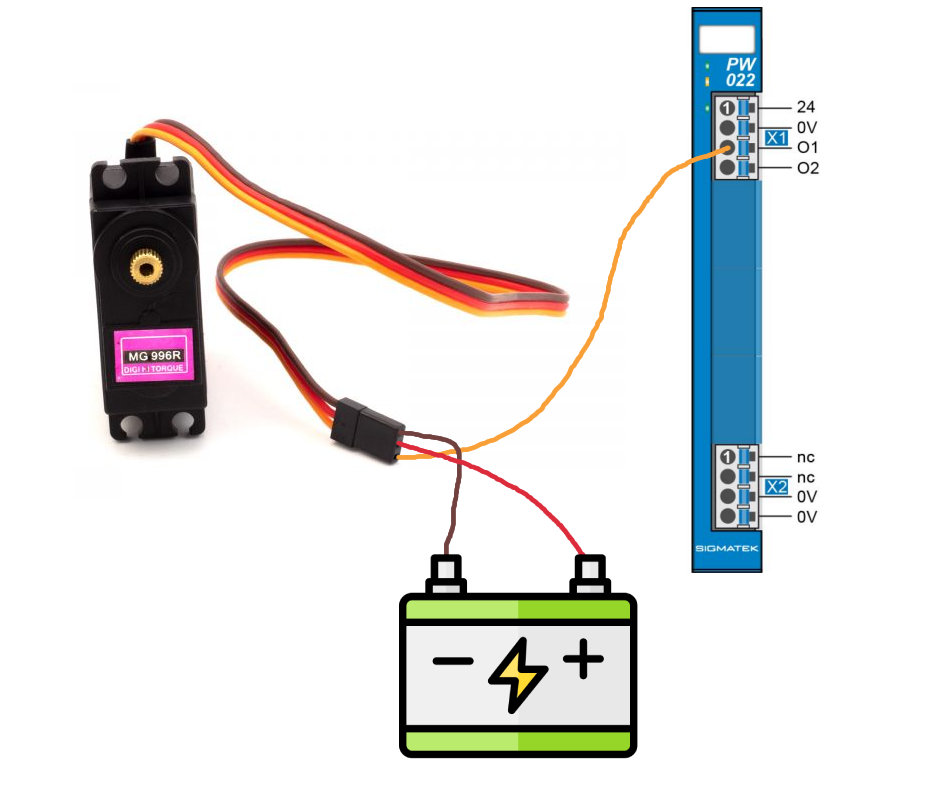
\includegraphics[width=0.7\columnwidth]{img/experiment/pw022_minirobot.png}
	\caption[Connection between PW 022 and mini-robot]{Connection between PW 022 and mini-robot~\cite{MG996RDigitalServo}}
	\label{fig:pw022_minirobot_connection}
\end{figure}

\begin{comment}
battery -> https://www.flaticon.com/de/kostenloses-icon/autobatterie_4238252?related_id=4238254
\end{comment}

\noindent The program was written in Lasal Class 2 and was applied to all three mentioned versions of Salamander 4 to measure the reaction time of the robot to the specific commands. Prior to examining the software program, the next two subsections briefly explain the setup of each version of the experiment.

\section{Setup of Hardware Salamander 4}
In this version, Salamander 4 runs on the CP 841~\cite{CPUEinheitenSIGMATEK} CPU unit, specifically designed for the Salamander 4 operating system. The PW 022 module is directly mounted on the CPU via the S-DIAS bus and communicates over the hard real-time capable Ethernet VARAN with 100 Mbit/s~\cite{SDIASSIGMATEK}. The setup is visible on Figure~\ref{fig:hardware_tree}.

\begin{figure}[H]
	\centering
	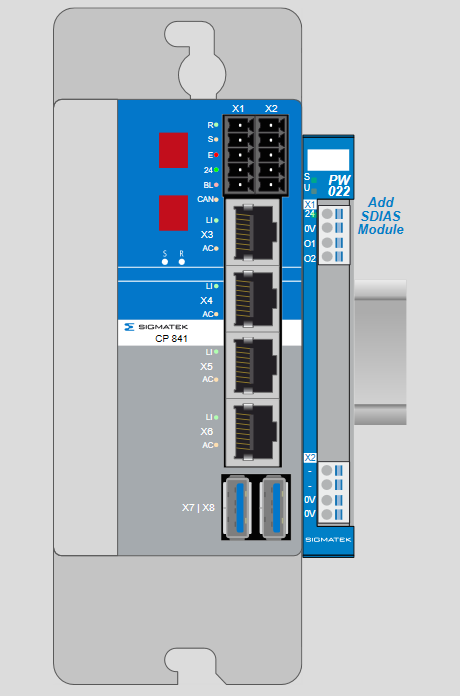
\includegraphics[width=0.5\columnwidth]{img/experiment/hardware_tree.png}
	\caption[Hardware tree]{Hardware tree}
	\label{fig:hardware_tree}
\end{figure}

\section{Setup of QEMU Salamander 4}\label{sec:setup_experiment_virtualized}
In the virtualized setup of the experiment, the VCPU functionality of QEMU is used to connect QEMU with the PWM module. In order to achieve that, the PCV 522 VARAN Manager PCI Insert Card~\cite{ControlsHMIsSIGMATEK}, which serves as a bridge between the PC and the rest of the setup, needed to be plugged into the PC. The command \texttt{lspci -nn} lists all PCI devices along with their vendor and device IDs. In this case, the command for binding the PCV 522 module to the VFIO-PCI driver was \texttt{sudo sh -c 'echo "5112 2200" > /sys/bus/pci/drivers/vfio-pci/new\_id'} with vendor ID 5112 and device ID 2200.  To verify that the device has been successfully bound to the VFIO-PCI driver, \texttt{lspci -v} can be used. On top of the binding process, the QEMU script from the previous sections also needed to be modified to include the PCV 522 VARAN Manager PCI Insert Card. This is done by adding \texttt{-device\ vfio-pci,host=03:00.0 } to the QEMU script, where \texttt{03:00.0} refers to the PCI address of the device, with \texttt{03} being the bus number, \texttt{00} the device number, and \texttt{0} the function number. The final script can be seen in Code~\ref{script:qemu_def_pci}.

\vspace{1em}
\begin{minipage}{\linewidth}
	\begin{lstlisting}[name={Include PCI in QEMU script for Salamander 4 virtualization},label={script:qemu_def_pci}]
	#!/bin/sh

	if  [ ! -d drive-c/ ]; then
					echo "Filling drive-c/"
					mkdir drive-c/
					tar -C drive-c/ -xf stek-drive-c-image-sigmatek-core2.tar.gz
	fi
		
	exec taskset -c 4-5 chrt -f 99 qemu-system-x86_64 -M pc,accel=kvm -kernel ./bzImage \
	-m 2048 -drive file=salamander-image-sigmatek-core2.ext4,format=raw,media=disk \
	-append "console=ttyS0 console=tty1 root=/dev/sda rw panic=1 sigmatek_lrt.QEMU=1 ip=dhcp rootfstype=ext4 schedstats=enable nohlt idle=poll quiet xeno_hal.smi=1 xenomai.smi=1 threadirqs" \
	-net nic,model=e1000,netdev=e1000 -netdev bridge,id=e1000,br=nm-bridge \
	-fsdev local,security_model=none,id=fsdev0,path=drive-c -device virtio-9p-pci,id=fs0,fsdev=fsdev0,mount_tag=/mnt/drive-C \
	-device vhost-vsock-pci,guest-cid=3,id=vsock0 \
	-drive if=pflash,format=qcow2,file=ovmf.code.qcow2 \
	-object memory-backend-ram,id=ram0,size=4G,prealloc=on \
	-mem-prealloc -mem-path /dev/hugepages \
	-device vfio-pci,host=03:00.0 \
	-no-reboot -nographic
\end{lstlisting}
\end{minipage}

\noindent An additional Varan Connection module VI 021~\cite{InterfacesSplittersSIGMATEK} was required to enable the connection between the PCV 522 module and the PW 022 module that generates the signal to move the mini-robot. This setup is depicted in Figure~\ref{fig:virt_tree}.

\begin{figure}[H]
	\centering
	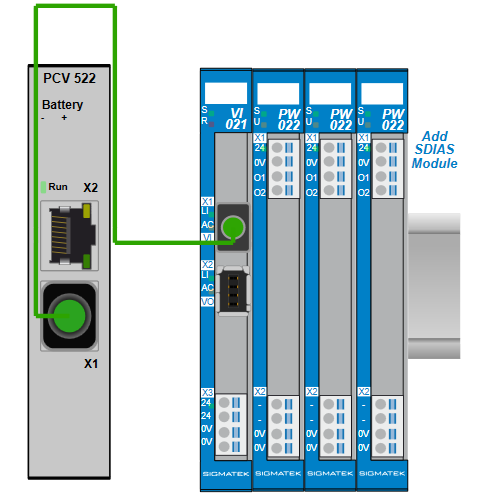
\includegraphics[width=0.5\columnwidth]{img/experiment/virt_tree.png}
	\caption[Virtualization tree]{Virtualization tree}
	\label{fig:virt_tree}
\end{figure}

\noindent Essentially, the CP 841 CPU is being emulated by the VCPU functionality of QEMU, allowing the PCV 522 VARAN Manager PCI Insert Card and the Varan Connection module VI 021 to interact as if they were communicating with a physical CPU unit.

\clearpage
\section{Robotic Application}

\clearpage

\begin{comment}
\chapter{To Include}\label{cha:to_include}

``korrekt''

\noindent \enquote{This LaTeX.}

The latency was measured under two conditions, idle and CPU-stressed. Vorgehensweise von~\cite{linPerformanceEvaluationXenomai}

\section{Trace-cmd and Kernelshark}
After analyzing the inital latency of both versions, Trace-cmd and Kernelshark were used to further inspect the reasons that caused this divergence.

\section{Host and Guest tasks}
\begin{table}[H]
	\centering
	\begin{minipage}{.5\textwidth}
		\centering
		\caption{Host report CPU19 (Total of 445.908)}
		\label{tab:results_host_report}
		\begin{tabular}{|c|c|c|}
			\hline
			PID    & Task                          & Count   \\ \hline
			182579 & qemu-system-x86               & 302.748 \\ \hline
			0      & \textless{}idle\textgreater{} & 112.911 \\ \hline
			182618 & vhost                         & 21.204  \\ \hline
			182572 & qemu-system-x86               & 7.597   \\ \hline
			182755 & qemu-system-x86               & 644     \\ \hline
			182754 & qemu-system-x86               & 643     \\ \hline
			181870 & kworker/19:1                  & 139     \\ \hline
			3820   & kworker/19:1H                 & 16      \\ \hline
			94     & migration/19                  & 6       \\ \hline
		\end{tabular}
	\end{minipage}%
	\begin{minipage}{.5\textwidth}
		\centering
		\caption{Guest report (Total of 362.370)}
		\label{tab:results_guest_report}
		\begin{tabular}{|c|c|c|}
			\hline
			PID & Task                          & Count   \\ \hline
			0   & \textless{}idle\textgreater{} & 150.744 \\ \hline
			331 & LRT-Main                      & 56.697  \\ \hline
			377 & trace-cmd                     & 48.507  \\ \hline
			346 & CLI                           & 26.426  \\ \hline
			378 & kthreadd                      & 25.837  \\ \hline
			340 & MainTaskLow                   & 19.291  \\ \hline
			339 & \textless{}...\textgreater{}  & 9.980   \\ \hline
			34  & MainTaskHigh                  & 9.185   \\ \hline
			327 & LE-Logger                     & 4.965   \\ \hline
			369 & kworker/0:0                   & 2.793   \\ \hline
			321 & kWorker-LRT                   & 2.542   \\ \hline
			328 & LRTMgr-Main                   & 1.651   \\ \hline
			34  & LrtMgrCyclic                  & 1.220   \\ \hline
			332 & cobalt\_printf                & 1.112   \\ \hline
			325 & LE-System                     & 534     \\ \hline
			343 & TCP-Listen                    & 187     \\ \hline
			15  & rcu\_preempt                  & 162     \\ \hline
			25  & kcompactd0                    & 122     \\ \hline
			58  & kworker/0:1H                  & 96      \\ \hline
			63  & kworker/u2:2                  & 89      \\ \hline
			8   & jbd2/sda-8                    & 86      \\ \hline
			22  & kworker/0:1                   & 56      \\ \hline
			1   & init                          & 31      \\ \hline
			2   & kthreadd                      & 25      \\ \hline
			375 & trace-cmd                     & 24      \\ \hline
			14  & ksoftirqd/0                   & 8       \\ \hline
		\end{tabular}
	\end{minipage}
\end{table}

\noindent In the following, the host and guest tasks along with their impact on system latency are briefly described.

\begin{itemize}
	\item \textbf{qemu-system-x86}: Part of the QEMU process and specifically, this task emulates x86 systems. In Table~\ref{tab:results_host_report}, it occurs four times under different PIDs, hence there are four threads of it.
	\item \textbf{<idle>}: This represents the idle time of the CPU, hence it is not being used by any process, allowing to save power. The system halts until the next interrupt, which could be a timer interrupt, I/O interrupt, etc.
	\item \textbf{vhost}: A kernel module which improves virtual input/output (virtio) performance by handling virtqueues in the kernel, thereby reducing context switches and system calls.
	\item \textbf{kworker/19:1}: A kernel worker thread created by the Linux kernel, kworker/19:1 performs work in response to system events. The number after the slash and colon indicate the CPU core and internal ID of the worker thread, respectively.
	\item \textbf{kworker/19:1H}: Similar to kworker/19:1, kworker/19:1H is a kernel worker thread, with the ‘H’ suggesting that this thread handles hardware interrupts.
	\item \textbf{migration/19}: The migration process is a kernel process that balances load across CPU cores by moving threads from one CPU to another. The number after the slash indicates the CPU core to which the migration process is bound. (URL: \url{https://elixir.bootlin.com/linux/latest/source/kernel/sched/core.c#L2325})

\end{itemize}

The Figure below (deleted) compares non-optimized guest latency with optimized guest latency and includes optimized bare-metal latency as a reference. The data shows that a 40\% reduction in QD1 latency is achievable through system tuning.

\section{Citation table}
\begin{table}[H]
	\centering
	\begin{tabular}{|p{0.1\textwidth}|p{0.45\textwidth}|p{0.45\textwidth}|}
		\hline
		\textbf{Number}                    & \textbf{Book} & \textbf{Citation} \\
		\hline
		\cite{maPerformanceTuningKVMbased} & book          & citation          \\
		\hline
		\cite{maPerformanceTuningKVMbased} & book          & citation          \\
		\hline
		\cite{maPerformanceTuningKVMbased} & book          & citation          \\
		\hline
		\cite{maPerformanceTuningKVMbased} & book          & citation          \\
		\hline
	\end{tabular}
	\caption{Your Caption}
	\label{tab:my_label}
\end{table}
\clearpage
\end{comment}

\chapter{Results}\label{cha:results}

Online

~\cite{pixelartSIGMATEKKompletteAutomatisierungssysteme}
~\cite{Tracecmd}
~\cite{KernelShark}
~\cite{XenomaiXenomai}
~\cite{CPUEinheitenSIGMATEK}
~\cite{EngineeringToolLASAL}
~\cite{WelcomeYoctoProject}
~\cite{QEMU}
~\cite{RealtimePreempt_rt_versionsWiki}
~\cite{RealtimeKernelPatchset}
~\cite{rostedtInternalsRTPatch}
~\cite{WhatRealtimeLinux}
~\cite{LinuxProcessPriorities}
~\cite{kernelrecipesKernelRecipes20162016}
~\cite{thelinuxfoundationFindingSourcesLatency2020}
~\cite{thelinuxfoundationChecklistWritingLinux2020}
~\cite{HOWTOBuildRTapplication}
~\cite{RealtimeProgrammingLinux}
~\cite{KVMQemuVirtualization}
~\cite{MG996RServoMotor}
~\cite{DigitalOutputSIGMATEK}
~\cite{MG996RDigitalServo}
~\cite{SDIASSIGMATEK}
~\cite{ControlsHMIsSIGMATEK}
~\cite{InterfacesSplittersSIGMATEK}
~\cite{lutsykPipelinedMulticoreMachine2020}
~\cite{CPUUnitsSIGMATEK}


\noindent Papers

~\cite{RealTimePerformanceTuning2022}
~\cite{maPerformanceTuningKVMbased}
~\cite{kiszkaLinuxRealTimeHypervisor}
~\cite{deoliveiraDemystifyingRealTimeLinux}
~\cite{mckenneyRealTimeVs}
~\cite{yoonRealTimePerformanceAnalysis}
~\cite{huang2015performance}
~\cite{junzhangPerformanceAnalysisKVMBased2010}
~\cite{perneelRealtimeCapabilitiesStandard2015}
~\cite{scordinoRealTimeVirtualizationIndustrial2020}

~\cite{broskyShieldedProcessorsGuaranteeing2003}
~\cite{adamRealTimePerformanceResponse2021}
~\cite{pielAsymmetricSchedulingLoad2006}
~\cite{malallahComprehensiveStudyKernel2021}
~\cite{queirozTestingLimitsGeneralpurpose2023}
~\cite{cinqueVirtualizingMixedCriticalitySystems2022}
~\cite{guStateoftheArtSurveyRealTime2012}
~\cite{javierperezHowRealTime2022}
~\cite{kirovaImpactModernVirtualization2019}
~\cite{REALTIMEOPERATING}
~\cite{garcia-vallsChallengesRealtimeVirtualization2014}
~\cite{masrurVMBasedRealTimeServices2010}

~\cite{HardRealTime}
~\cite{adamPerformanceAssessmentLinux2021}
~\cite{jiangRealTimeSystemManycore}
~\cite{wangRealtimeEmbeddedSystems2017}
~\cite{lipariRealTimeSchedulingHard}
~\cite{canbazPerformanceAnalysisRealtime2022}
~\cite{reghenzaniRealTimeLinuxKernel2020}
\clearpage

\chapter{Discussion}\label{cha:discussion}
\clearpage

\chapter{Summary and Outlook}\label{cha:summary_and_outlook}
\section{Trace-cmd \& Kernelshark}



%
% Hier beginnen die Verzeichnisse.
%
\clearpage
\printbibliography
\clearpage
% Das Abbildungsverzeichnis
\listoffigures
\clearpage

% Das Tabellenverzeichnis
\listoftables
\clearpage

% Das Quellcodeverzeichnis
\listofcode
\clearpage

\phantomsection
\addcontentsline{toc}{chapter}{\listacroname}

\chapter*{\listacroname}
\begin{acronym}[XXXXX]
	\acro{CPU}[CPU]{Central Processing Unit}
	\acro{QEMU}[QEMU]{Quick Emulator}
	\acro{IRQ}[IRQ]{Interrupt Request}
\end{acronym}

%
% Hier beginnt der Anhang.
%
\clearpage
\appendix
\begin{comment}
\chapter{Anhang A}
\clearpage
\chapter{Anhang B}
\end{comment}

\end{document}
